\documentclass{article}
%% \documentclass[dvipdfmx,a4paper]{article}


%%% macros
%%\input{narrowermargin} %% lncs contents with narrower margins
%%% begin: papersize with narrower margins
%% \usepackage[papersize={50mm,50mm}]{geometry}
%%% narrowmargin.tex
%%% begin: papersize with narrower margins
\usepackage{calc}
\newlength{\marginwidth} %% 
\newlength{\contentswidth} %% lncs
\newlength{\contentsheight} %% lncs
\newlength{\mypaperwidth} %% paper
\newlength{\mypaperheight} %% paper
\setlength{\marginwidth}{20mm} %% 
\setlength{\contentswidth}{145mm} %% lncs
\setlength{\contentsheight}{225mm} %% lncs
\setlength{\mypaperwidth}{\contentswidth+\marginwidth} %% paper
\setlength{\mypaperheight}{\contentsheight+\marginwidth} %% paper
\usepackage[papersize={\mypaperwidth,\mypaperheight},margin=\marginwidth]{geometry} 
%%% end: papersize 
%%% EOF

%% \input{myarith}
%%% end: papersize
\usepackage{amsmath,amssymb}
\usepackage{amsthm} %%proof environment
%%% auto labeling
\usepackage{mathtools}
\mathtoolsset{showonlyrefs=true}
%%% end: auto labeling
\usepackage{enumerate}
\usepackage{booktabs}
\usepackage{graphicx}
\graphicspath{
  {fig/}
  {fig/new/}
}%%画像のパス.末尾は'/'で終わること
%%%% algo
\usepackage[ruled,vlined,linesnumbered]{algorithm2e}
%%% setting: algorithm2e %%%%%%%%%%%%%%%%%%%%%%%%%%%%%%%%
\newcommand{\algoopts}{%
%%% RULES
%boxed,%good
%boxruled,%
%algoruled,%good
ruled,%
%tworuled,%
%%% CODE TYPESETTING
%% hangingcomment,%
%% opthanginginout,%
%% noalgohanging,%obsolute 
%%% BLOCKS DISPLAY
%noline,%
vlined,%L-tyle
%lined,%I-style
%%%
linesnumbered%
}
%%\usepackage[\algoopts]{algorithm2e} 
\usepackage[ruled,vlined,linesnumbered]{algorithm2e} 

\makeatletter
\renewcommand{\@algocf@capt@plain}{above}% formerly {bottom}
\makeatother
%%% algorithm2e
\newcommand{\comblk}[1]{\hfill$\rhd$\ \textit{#1}}
\newcommand{\Commentblock}[1]{\comblk{#1}}
\newcommand{\Commentblockl}[1]{\kern0.5em$\rhd$\ \textit{#1}\ $\lhd$}
\newcommand{\CM}[1]{\comblk{#1}}
%% \SetArgSty{textrm}%arguments for e.g., if, else, while etc. 
%% \SetCommentSty{textit}%arguments for comments
\SetKwComment{Comment}{$\rhd$}{} 
\SetKwInput{KwInput}{Input}
\SetKwInput{KwOutput}{Output}
\SetKwInput{KwNotes}{Notes}
%%%
\SetKwInput{KwPreproc}{Preprocess}
\SetKwInput{KwRuntime}{Runtime}
\SetKwInput{KwGiven}{Given}
\SetKwInput{KwGlobal}{Global}
\SetKwInput{KwWork}{Working}
\SetKwInput{KwMethod}{Method}
\SetKwInput{KwPrecond}{Pre-condition}
\SetKwInput{KwPostcond}{Post-condition}
\SetArgSty{textrm}%arguments for e.g., if, else, while etc. 
\SetCommentSty{textit}%arguments for comments
\newcommand{\iIf}[2]{\textbf{if} {#1} \textbf{then}\hspace{0.125em}{\relax #2}}
\newcommand{\iElseIf}[2]{\textbf{else if} {#1} \textbf{then}\hspace{0.125em}{\relax #2}}
\newcommand{\iElse}[1]{\textbf{else} {\relax #1}}
\newcommand{\iFor}[2]{\textbf{for} {#1} \textbf{do}\hspace{0.125em}{\relax #2}}



%%%
%% \usepackage{natbib}
%\setcitestyle{numbers,super}
%%%
\usepackage{tikz}
\usetikzlibrary{calc}
%\usetikzlibrary{intersections,calc,arrows.meta}

%%% macro private
%%% config.tex

%%======================================
\usepackage{graphicx}
%% \usepackage{amsmath,amssymb}
%% \usepackage{mathtools}
%% \mathtoolsset{showonlyrefs=false} %% 参照している式参照のみ表示
%% \mathtoolsset{showonlyrefs=true} %% 参照している式参照のみ表示
%% \usepackage{cite}
\usepackage{caption}    %%for subfigure
\usepackage[skip=0.5ex]{subcaption} %%for subfigure
\captionsetup{aboveskip=0.0\baselineskip}
\captionsetup{belowskip=0.0\baselineskip}
%%%
%%\usepackage{titlesec}
%% \titlespacing*{\section}{0pt}{5.5ex plus 1ex minus .2ex}{4.3ex plus .2ex}
%% \titlespacing*{\subsection}{0pt}{5.5ex plus 1ex minus .2ex}{4.3ex plus .2ex}

%%% table
%% \usepackage{multirow}
\usepackage{booktabs}
\usepackage{array}

% private macros by others 
\usepackage{url}
\usepackage{bm}
\usepackage{textcomp}%%for cent
%\usepackage[margin=1.75in]{geometry}
%\usepackage[margin=1.0in]{geometry}
%% \usepackage{subfig}
%% \usepackage{natbib}

%%% private %%%%%%%%%%%%%%%%%%%%%%%%%%%%%%%%%%%%%

%% private macros by arim@ist
%%% jsvmac.tex
%%% macros from a subset of jsv1.sty 

%%% from jsv1.sty

% Write multichar identifier names using \id in either mathmode or text;
% For ex, $\id{high}(x)$ is an expression using the \id{high} function.
% Use ``\ '' if a space is desired, as in math mode.
\def\id#1{\ensuremath{\mathit{#1}}}
\let\idit=\id
\def\idbf#1{\ensuremath{\mathbf{#1}}}
\def\idrm#1{\ensuremath{\mathrm{#1}}}
\def\idtt#1{\ensuremath{\mathtt{#1}}}
\def\idsf#1{\ensuremath{\mathsf{#1}}}
\def\idcal#1{\ensuremath{\mathcal{#1}}}  % Use with capital letter args only
\def\idsc#1{\ensuremath{\textsc{#1}}} % added by arim

%%% end jsv1.sty

%%% EOF

%%\input{arimmacro} %%privatemacro


%%%%%%%%%%%%%%%%%%%%%%%%%%%%%%%%%%%%%%%%
%%xsavebox
\usepackage{xsavebox}

%%%%%%%%%%%%%%%%%%%%%%%%%%%%%%%%%%%%%%%%%
%%% above and below float figure table
\setlength\intextsep{0.5\baselineskip}
\setlength\abovecaptionskip{0.0\baselineskip}
\setlength\belowcaptionskip{0.5\baselineskip}
%% \setlength\intextsep{18pt}

%%%%%%%%%%%%%%%%%%
%% latex native savebox and lrbox
\newenvironment{savethm}[1]{\begin{lrbox}{#1}\begin{minipage}[t]{1.0\textwidth}}{\end{minipage}\end{lrbox}}

\newcommand{\putthm}[1]{
%% \smallskip
\noindent 
\usebox{#1}
\medskip}

%%sample
%% \newsavebox{\thmbox}
%% \begin{lrbox}{\thmbox}
%% \begin{minipage}[t]{1.0\textwidth}
%% \begin{theorem}\label{thm:algbwt:main}
%% ....
%% \end{theorem}
%% \end{minipage}
%% \end{lrbox}


%% \putthm{\thmbox}


%%%%%%%%%%%%%%%%%%




%%%%%%%%%%%%%%%%%%%%%%%%%%%%%%%%%%%%%%%%
%%comment out a paragraph
\newsavebox{\cmbox}
\newenvironment{commbox}{
  \begin{lrbox}{\cmbox}
    \begin{minipage}{.9\textwidth}
}{\end{minipage}
  \end{lrbox}
  %\framebox{\usebox{\cmbox}}
}


%%%%%%%%%%%%%%%%%%%%%%%%%%%%%%%%%%%%%%%%
% %%% empty environment 
% \newenvironment{myempty}{\begin{commbox}}{\end{commbox}}
% %%% proof environment 
% \newenvironment{myproof}{\begin{proof}}{\end{proof}} %default
% \newenvironment{myfullproof}{\begin{proof}}{\end{proof}} %default
% \newenvironment{myfullproofempty}{\begin{myempty}}{\end{myempty}} %default

%% replace an enviroment #1 with #2
\newcommand{\myenvironmentreplace}[2]{\renewenvironment{#1}{\begin{#2}}{\end{#2}}}

%% claim %%
\newenvironment{myclaim}[1][]{\bgroup\parskip=0mm\par (\textit{Claim{#1}})}{(\textit{End of Claim})\par\egroup}  
\newenvironment{proofofclaim}{\bgroup\parindent=1em\parskip=0mm\par (\textit{Proof for the claim})}{(\textit{End of the proof for the claim})\par\egroup}  
\newenvironment{proofofclaimempty}{\begin{myempty}}{\end{myempty}}

%% \newenvironment{proofofclaim}{\bgroup\parskip=0mm\par (Proof for the claim)}{(End of the proof for the claim)\par\egroup}  


%%%%%%%%%%%%%%%%%%%%%%%%%%%%%%%%%%%%%%%%

% %% switch catcode of '&' between 4 and 9
% \newenvironment{inalign}{\begin{math}\catcode`&=9}{\catcode`&=4\end{math}}

%%%%%%%%%%%%%%%%%%%%%%%%%%%%%%%%%%%%%%%%

% lipics predefined

%% send a proof to the appendix
\newtheorem{definition}{Definition}
\newtheorem{theorem}{Theorem}
\newtheorem{lemma}[theorem]{Lemma}
\newtheorem{proposition}{Proposition}
\newtheorem{corollary}[theorem]{Corollary}
\newtheorem{remark}{Remark}
\newtheorem{fact}{Fact}
\newtheorem{condition}{Condition}

% \newtheorem{example}[example]{Example}[section]
% \newtheorem{conjecture}{Conjecture}
% %% dammy
%%%%%%%%%%%%%%%%%%%%%%%%%%%%%%%%%%%%%%%%

%%% cleveref
\usepackage{cleveref}
\crefname{section}{Sec.}{Sections}
\crefname{chapter}{Chapter}{Chapters}
%%
\crefname{algorithm}{Algorithm}{Algorithms}
\crefname{table}{Table}{Tables}
\crefname{figure}{Fig.}{Figures}
%% 
\crefname{definition}{Definition}{Definitions}
\crefname{lemma}{Lemma}{Lemmas}
\crefname{proposition}{Prop.}{Propositions}
\crefname{theorem}{Theorem}{Theorems}
\crefname{remark}{Remark}{Remarks}
\crefname{fact}{Fact}{Facts}
\crefname{condition}{Condition}{Conditions}
\crefname{problem}{Problem}{Problems}
\crefname{observation}{Observation}{Observations}
%% \crefname{lemma}{Lemma}{Lemmas}
\crefname{equation}{Eq.}{Equations}
%%% fix of a bug in Algorithm
\newcommand{\aref}[1]{Algorithm\kern0.25em\ref{#1}} 
%%%%%%

% %% send a proof to the appendix
\usepackage{apxproof}
% \newtheoremrep{definition}{Definition}[section]
\newtheoremrep{lemma}[theorem]{Lemma}[section]
\newtheoremrep{proposition}[proposition]{Proposition}[section]
\newtheoremrep{theorem}[theorem]{Theorem}[section]
\newtheoremrep{corollary}[theorem]{Corollary}[section]
% \newtheoremrep{remark}[theorem]{Remark}

%% \newtheoremrep{example}[example]{Example}[section]
%% \newtheoremrep{conjecture}{Conjecture}
%% %% dammy
%% \newcommand{\resetrep}{}
%% rest 
%% \newcommand{\resetreptext}{{\rm\textsf{in draft}}}
%% \newcommand{\getfollow}[1][{}]{{\rm\textsf{(*{#1})}}\ }

%% \newcommand{\resetrep}{%% resetting all rep-style environments
%% %% \renewenvironment{lemmarep}{\begin{lemma}\getfollow}{\end{lemma}}
%% \renewenvironment{lemmarep}{\begin{lemma}\getfollow}{\end{lemma}}
%% \renewenvironment{propositionrep}{\begin{proposition}\getfollow}{\end{proposition}}
%% \renewenvironment{theorem}{\begin{theorem}\getfollow}{\end{theorem}}
%% \renewenvironment{corollaryrep}{\begin{corollary}\getfollow}{\end{corollary}}
%% \renewenvironment{examplerep}{\begin{example}\getfollow}{\end{example}}
%% \renewenvironment{remarkrep}{\begin{remark}\getfollow}{\end{remark}}
%% \renewenvironment{conjecturerep}{\begin{conjecture}\getfollow}{\end{conjecture}}
%% \renewenvironment{toappendix}{}{}
%% }

%%%%% 
\newenvironment{statement}[1]{\begin{trivlist}\item[]$\blacktriangleright\:$\textbf{#1}\ }{\end{trivlist}}
\newenvironment{notoappendix}{}{} %% the empty version of toappendix

%%%%%%%%%%%%%%%%%%%%%%%%%%%%%%%%%%%%%%%%%
%% enumitem: smart enumerate and itemize
%% the vspace above list = \topsep + \parskip + \partopsep
%% the vspace between items = \itemsep + \Parsep 
%% the vspace between paragraphs = \Parsep 
\usepackage[inline,shortlabels]{enumitem} %enumerate
\setlist{noitemsep}
\setlist{%
topsep = 0.25\baselineskip,
parsep = 0.125\baselineskip
}%exp
\setlist[enumerate]{ labelsep=.25pc, leftmargin=1.5pc } 
%% \setlist[enumerate]{ labelsep=.25pc, leftmargin=1.5pc } 
\setlist[enumerate,1]{ label= (\arabic*), ref=\arabic*}
\setlist[enumerate,2]{ label= (\roman*),ref  = \roman*}
\setlist[enumerate,3]{ label= (\alph*), ref  = (\alph*)}
%\setlist[itemize]{ leftmargin=1.5pc }
\setlist[description]{ font=\sffamily\bfseries }
%% end macros
%%% switch
%% \newenvironment{myenumerate}{\begin{enumerate}}{\end{enumerate}}
\newenvironment{myenumerate}{\begin{enumerate*}}{\end{enumerate*}}
%% end macros

%%

%% %% 目次のハイパーリンク: 印刷時は念の為コメントアウト(本来出ない)
%% \usepackage[%
%% %dvipdfmx,%
%% colorlinks=true,%
%% linkcolor=blue,%
%% anchorcolor=black,%
%% citecolor=blue,%
%% urlcolor=blue%
%% ]{hyperref} %注意:パッケージの最後に読み込むこと

%%%%

%% EOF

%%% 数式モードで使う表記
\newcommand{\set}[1]{\{#1\}}
\newcommand{\iffdef}{\stackrel{\idrm{def}}{\iff}}
\renewcommand{\mod}{\idrm{mod}}
\newcommand{\Key}[1]{\Statex\hspace{-1.2\leftmargin}  \textbf{#1}\hspace{.25em}}
\newcommand{\Proc}[1]{\Key{Procedure}{#1}}
%\newcommand{\Proc}[1]{\Statex\hspace{-1.2\leftmargin}  \textbf{Procedure}\hspace{.25em}{#1}}
\newcommand{\ename}[2]{\textbf{#1} (\textit{#2})}
\newcommand{\itl}[1]{\textit{#1}}
\newcommand{\sig}[1]{\mathcal{#1}}

%%% 数式モードで文字が開く問題を解消する機能

\def\id#1{\ensuremath{\mathit{#1}}}
\let\idit=\id
\def\idbf#1{\ensuremath{\mathbf{#1}}}
\def\idrm#1{\ensuremath{\mathrm{#1}}}
\def\idtt#1{\ensuremath{\mathtt{#1}}}
\def\idsf#1{\ensuremath{\mathsf{#1}}}
\def\idcal#1{\ensuremath{\mathcal{#1}}} 

%%% 参照の便利版
\usepackage{cleveref}
\crefname{algorithm}{アルゴリズム}{Algorithms}
\crefname{table}{表}{Tables}
\crefname{figure}{図}{Figures}
\crefname{section}{節}{Sections}
\crefname{chapter}{章}{Chapters}
\crefname{problem}{問題}{Problems}
\crefname{definition}{定義}{Definitions}
\crefname{lemma}{補題}{Lemmas}
\crefname{fact}{事実}{Facts}
\crefname{property}{性質}{Properties}
\crefname{proposition}{命題}{Propositions}
\crefname{thmeorem}{定理}{Theorems}
\crefname{cor}{系}{Corollaries}
\crefname{footnote}{脚注}{Footnotes}
%%% notation.tex


%%%% new atoc 
\newcommand{\Sub}{\idsf{Sub}}
%% \newcommand{\Suf}{\idsf{Suf}}
%% \newcommand{\Pref}{\idsf{Pref}}
\newcommand{\LPF}{\idrm{LPF}}

\newcommand{\SA}{\idrm{SA}}
\newcommand{\ISA}{\idrm{ISA}}
\newcommand{\LCP}{\idrm{LCP}}
\newcommand{\BWT}{\idrm{BWT}}

%%%%

%%% algo
\newcommand{\RecLPT}{\textsf{RecLPT}}  %% TDSA
\newcommand{\RecCDAWG}{\textsf{RecCDAWG}}  %% TDSA
\newcommand{\SkipAndCount}{\textsf{SkipAndCount}}  %% TDSA
\newcommand{\FindNonEquivLocus}{\textsf{FindLongestPrefixPath}}  %% TDSA

\newcommand{\MREnum}{\textsf{Enum}}  %% TDSA
\newcommand{\GenChildren}[1][{\LCP}]{\textsf{GenChildren}_{#1}}  
\newcommand{\ColoredRange}[1][{\BWT,RMQ}]{\textsf{ColoredRange}_{#1}}  
\newcommand{\append}{\op{append}}

\newcommand{\LChar}[1][S]{\idrm{LChar}_{#1}}
\newcommand{\RChar}[1][S]{\idrm{RChar}_{#1}}
\newcommand{\getfactor}[1][{\SA, S}]{\op{Fact}_{#1}} 
\newcommand{\isLeftBranching}[1][{\SA, \ISA, S}]{\proc{isLeftBranching}_{#1}}\newcommand{\RREP}{\mathcal{RP}}  %% TDSA

%%%
%% \newcommand{\rk}[1]{^{(#1)}} %%alias 
\newcommand{\idx}[3]{_{#1=#2}^{#3}} %%alias
%% \newcommand{\btw}[3]{{#2}\le {#1}\le {#3}} %%alias
%% \newcommand{\Suf}{\idrm{Suf}}
%% \newcommand{\Fac}{\idrm{Fac}}

%%%%  orig
\newcommand{\loc}[1]{\underline{#1}}
\newcommand{\lab}{\idtt{label}}
\newcommand{\src}{\idtt{src}}
\newcommand{\dst}{\idtt{dst}}
\newcommand{\str}{\idtt{str}}
\newcommand{\Spos}[1][S]{\idtt{Spos}_{#1}}
\newcommand{\Epos}[1][S]{\idtt{Epos}_{#1}}
\newcommand{\eqspos}[1][S]{\equiv^{#1}_{spos}}
\newcommand{\eqepos}[1][S]{\equiv^{#1}_{epos}}
\newcommand{\EQCspos}[1]{[{#1}]_{\eqspos}}
\newcommand{\EQCepos}[1]{[{#1}]_{\eqepos}}
%% \newcommand{\In}[1][G]{E^\idrm{in}_{#1}}
%% \newcommand{\Out}[1][G]{E^\idrm{out}_{#1}}
\newcommand{\In}[1][G]{\idrm{In}_{#1}}
\newcommand{\Out}[1][G]{\idrm{Out}_{#1}}
\newcommand{\ldep}{\op{ldep}}
\newcommand{\sdep}{\op{sdep}}
\renewcommand{\suf}{\id{suf}}
\newcommand{\wlink}{\id{wlink}}
\newcommand{\succeqsuf}{\succeq^\idrm{suf}}
\newcommand{\succsuf}{\succ^\idrm{suf}}
%\newcommand{\lex}{\idrm{lex}}

%%%
\newcommand{\CDAWG}[1][S]{\idrm{CDAWG}}
\newcommand{\Stree}[1][S]{\idrm{Stree}}
\newcommand{\LPT}[1][+]{\idsf{LPT}_{#1}}
\newcommand{\LPTrm}[1][+]{LPT$_{#1}$}
\newcommand{\LPTplus}{\LPT[+]}
\newcommand{\LPTminus}{\LPT[-]}
\newcommand{\source}[1][G]{\idrm{source}_{#1}}
\newcommand{\sink}[1][G]{\idrm{sink}_{#1}}
\newcommand{\Path}[1][G]{\idsf{Path}_{#1}}
\newcommand{\String}[1][G]{\idsf{String}_{#1}}
\newcommand{\para}[2][]{\idsc{#2}_{#1}}
\newcommand{\snd}[2][]{{#2}^\idrm{snd}_{#1}}
%% \newcommand{\Esnd}[1][]{E^\idrm{2nd}_{#1}}
\newcommand{\Esnd}[1][]{\snd[LPF]{E}}
\newcommand{\PATHsnd}[1][]{\snd[LPF]{Path}}

\newcommand{\svalue}[1][]{\idtt{value}_{#1}}
\newcommand{\ReplPref}[1][]{\idtt{value}^\idrm{pref}_{#1}}
\newcommand{\ReplSuf}[1][]{\idtt{value}^\idrm{suf}_{#1}}
\newcommand{\ReplPath}[1][]{\idsc{Path}^\idrm{repl}_{#1}}
%% \newcommand{\ReplPref}[1][]{\idsc{pref}^\idrm{repl}_{#1}}
%% \newcommand{\ReplSuf}[1][]{\idsc{suf}^\idrm{repl}_{#1}}
%% \newcommand{\ReplPath}[1][]{\idsc{Path}^\idrm{repl}_{#1}}

\newcommand{\pos}[1][]{\idtt{pos}_{#1}}
\newcommand{\val}[1][]{\idtt{val}_{#1}}
\newcommand{\Value}[1][S]{\idtt{value}_{#1}}
%%% 
\newcommand{\lext}[2][S]{\overleftarrow{#2}^{#1}} 
\newcommand{\rext}[2][S]{\overrightarrow{#2}^{#1}} 
\newcommand{\mext}[2][S]{\overleftrightarrow{#2}^{#1}}
\newcommand{\MR}{\textsf{MR}}
\newcommand{\RM}{\textsf{RM}}
\newcommand{\LM}{\textsf{LM}}
\newcommand{\M}{\MR}%%
\newcommand{\RR}[1][S]{\idcal{P}_{#1}}
\newcommand{\Parent}[1][S]{\idtt{Parent}_{#1}}
%%%%

\newcommand{\mysubsubsection}[1]{\textbf{#1}.\hspace{0.125em}}%% camera
\newcommand{\myfootnote}[1]{\hspace{-0.125em}\footnote{#1}}

%% macros.tex

%%%%%%%%%%%%%%%%%%%%%%%%%%%%%%%%%%%%%%%%%
%% reference with [] in environment 
\def\refbox(#1){$\mbox{\bf ({#1}) }$}
\newcommand{\mysubsubsection}[1]{\textbf{#1}.\hspace{0.125em}}%% camera
%% \newcommand{\mysubsection}[1]{\subsection*{#1}}

%% private macros: cdawg
%% class names
\newcommand{\suffix}{\id{Suffix}}
\newcommand{\substr}{\id{Substr}}
\newcommand{\prefix}{\id{Prefix}}
\newcommand{\Suf}{\suffix}
\newcommand{\Substr}{\substr}
\newcommand{\Pref}{\prefix}
%%% 
\newcommand{\lext}[1]{\overleftarrow{#1}} 
\newcommand{\rext}[1]{\overrightarrow{#1}} 
\newcommand{\mext}[1]{\overleftrightarrow{#1}}
\newcommand{\str}{\op{str}}
%%%
\newcommand{\spos}[1][S]{\op{Spos}_{#1}}
\newcommand{\epos}[1][S]{\op{Epos}_{#1}}
\newcommand{\occ}[1][]{\op{Occ}_{#1}}
%% maximal 
\newcommand{\RM}{\sig{RM}}
\newcommand{\LM}{\sig{LM}}
\newcommand{\M}{\sig{M}}
%%%%
\newcommand{\rstate}[1]{[{#1}]_{\equiv_R}}
\newcommand{\lstate}[1]{[{#1}]_{\equiv_L}}
%%%
\newcommand{\BUSA}{\textsf{BUSA}} 
\newcommand{\TDSA}{\textsf{TDSA}} 
\newcommand{\TDBW}{\textsf{TDBW}}
%%%
\newcommand{\MAW}{\idit{MAW}} 
\newcommand{\MUS}{\idit{MUS}} 
\newcommand{\MRW}{\idit{MRW}} 
\newcommand{\MRWK}[1][k]{\mbox{$#1$-\idit{MRW}}}
%%%%
%%% data structures
\newcommand{\stree}{\id{STree}}%exp
\newcommand{\weiner}{\id{Weiner}}%exp
\newcommand{\CDAWG}{\mathit{CDAWG}}
\newcommand{\SA}{\id{SA}}
\newcommand{\ISA}{\id{ISA}}
\newcommand{\BWT}{\id{BWT}}
\newcommand{\LCP}{\id{LCP}}
\newcommand{\LCE}[1][T]{\idrm{LCE}_{#1}}
%%%
\newcommand{\repr}{\op{repr}}
\newcommand{\intr}{\op{SA\textrm{-}Int}}
\newcommand{\lcpmin}{\op{lcpmin}}
%%%%
\newcommand{\set}[1]{\{\kern0.05em#1\kern0.05em\}}
\newcommand{\sete}[1]{\{\kern0.2em#1\kern0.2em\}}
\newcommand{\liste}[1]{[\kern0.2em#1\kern0.2em]}

%%%%
%\newcommand{\mywspace}[1][R]{O(\sigma^2\log e_{#1})}
%% \newcommand{\td}{\idsf{Td}}
%% \newcommand{\bu}{\idsf{Bu}}
%% \newcommand{\fw}{\idsf{Fwd}}
%% \newcommand{\bw}{\idsf{Bwd}}
\newcommand{\td}{\idsf{T}}
\newcommand{\bu}{\idsf{B}}
\newcommand{\fw}{\idsf{F}}
\newcommand{\bw}{\idsf{B}}
\newcommand{\tdfw}{\mbox{\td\fw}}
\newcommand{\tdbw}{\mbox{\td\bw}}
\newcommand{\bufw}{\mbox{\bu\fw}}
\newcommand{\bubw}{\mbox{\bu\bw}}
\newcommand{\tdfwd}{\tdfw}%% obsolute 
\newcommand{\tdbwd}{\tdbw}%% obsolute 
\newcommand{\bufwd}{\bufw}%% obsolute 
\newcommand{\bubwd}{\bubw}%% obsolute 
% %%% 

%%%%%%%%%%%%%%%%%%%%%%%%%%%%%%%%%%%%%%%%%
\usepackage{yhmath}%% for neat wide tilde

%%%%%%%%%%%%%%%%%%%%%%%%%%%%%%%%%%%%%%%%%

%% basis 
\renewcommand{\-}{\mbox{\textit{-}}}

%% symbols
\newcommand{\nat}{\mathbb{N}}
\newcommand{\rat}{\mathbb{R}}
\newcommand{\zat}{\mathbb{Z}}
\renewcommand{\leq}{\leqslant}%override
\renewcommand{\le}{\leqslant}%override
\renewcommand{\preceq}{\preccurlyeq}%override
\newcommand{\rev}{^\fn{rev}}

%% typeface 
\newcommand{\proc}[1]{\mbox{\textsf{#1}}}
\newcommand{\algo}[1]{\mbox{\textsf{#1}}}
\newcommand{\fn}[1]{\ensuremath{\mathrm{#1}}} 
\newcommand{\mb}[1]{\mathbb{#1}}
\newcommand{\name}[1]{\textit{#1}}

\newcommand{\eps}{\varepsilon}
\newcommand{\daller}{\$} %$
\renewcommand{\sharp}{\#} %$
\newcommand{\mathdaller}{\mbox{`$\daller$'}} %$
\newcommand{\centsymbol}{\mbox{\textcentoldstyle}} %$
\DeclareMathOperator{\polylog}{\mathrm{polylog}}

\newcommand{\kw}[1]{\textbf{#1}}
\newcommand{\sig}[1]{\mathcal{#1}}
\newcommand{\ty}[1]{\texttt{#1}}
%% \newcommand{\op}[1]{\mathtt{#1}}
%% \renewcommand{\-}{\mbox{-}}
\newcommand{\mop}[1]{\mbox{\rm\texttt{#1}}}%%exp
\newcommand{\op}[1]{\mathtt{#1}}


%% math: general 
\newcommand{\by}{\times}
\renewcommand{\bar}[1]{\overline{#1}}
\newcommand{\ceil}[1]{\lceil #1\rceil}
\newcommand{\floor}[1]{\lfloor #1\rfloor}
%\newcommand{\Implies}{\:\:}
\renewcommand{\iff}{\mathbin{\,\Leftrightarrow\,}}%override
\newcommand{\iffdef}{\mathbin{\,\stackrel{\textrm{def}}{\iff}\,}}
\newcommand{\Implies}{\mathbin{\,\Rightarrow\,}}%override
\newcommand{\To}{\Implies}%override
%% \newcommand{\iffshort}{\Leftrightarrow} %%short
\newcommand{\indicator}[1]{\mathbb{I}\kern-0.1em\left[\kern0.1em{#1}\kern0.1em\right]}
\newcommand{\pair}[1]{\langle #1\rangle}
%% \renewcommand{\mid}{\,:\,}
\newcommand{\infrac}[2]{{#1}\,/\,{#2}} %inline frac

%% not used 
\newcommand{\pow}[1]{2^{#1}}
\newcommand{\rng}[3]{_{#1=#2}^{#3}}
%% \renewcommand{\vec}[1]{\mathbf{#1}}
\newcommand{\rk}[1]{^{(#1)}}
\newcommand{\rkk}[1]{^{\kern.5pt\textrm{#1}}}


%%% tentative
\DeclareMathOperator{\pd}{..}
%%% tex hack: ".."コマンドを作成する
%%% https://tex.stackexchange.com/questions/4216/how-to-typeset-correctly
% \mathchardef\ordinarycolon\mathcode`\.
%%% raise: http://www.math.kobe-u.ac.jp/HOME/kodama/tips-latex-math-margin.html#raise 
\mathcode`\.=\string"8000
\begingroup \catcode`\.=\active
  \gdef.{\hbox{\hskip1pt\raise-2pt\hbox{$\cdot$\hskip1pt}}}
\endgroup
%%% end tex hack


%%% setting: algorithm2e %%%%%%%%%%%%%%%%%%%%%%%%%%%%%%%%
\newcommand{\algoopts}{%
%%% RULES
%boxed,%good
%boxruled,%
%algoruled,%good
ruled,%
%tworuled,%
%%% CODE TYPESETTING
%% hangingcomment,%
%% opthanginginout,%
%% noalgohanging,%obsolute 
%%% BLOCKS DISPLAY
%noline,%
vlined,%L-tyle
%lined,%I-style
%%%
linesnumbered%
}
%%\usepackage[\algoopts]{algorithm2e} 
\usepackage[ruled,vlined,linesnumbered]{algorithm2e} 

\makeatletter
\renewcommand{\@algocf@capt@plain}{above}% formerly {bottom}
\makeatother
%%% algorithm2e
\newcommand{\Commentblock}[1]{\hfill$\rhd$\ \textit{#1}}
\newcommand{\Commentblockl}[1]{\kern0.5em$\rhd$\ \textit{#1}\ $\lhd$}
\newcommand{\CM}[1]{\Commentblock{#1}}
%% \SetArgSty{textrm}%arguments for e.g., if, else, while etc. 
%% \SetCommentSty{textit}%arguments for comments
\SetKwComment{Comment}{$\rhd$}{} 
\SetKwInput{KwGiven}{Given}
\SetKwInput{KwGlobal}{Global}
\SetKwInput{KwWork}{Working}
\SetArgSty{textrm}%arguments for e.g., if, else, while etc. 
\SetCommentSty{textit}%arguments for comments
\newcommand{\iIf}[2]{\textbf{if} {#1} \textbf{then}\hspace{0.125em}{\relax #2}}
\newcommand{\iElseIf}[2]{\textbf{else if} {#1} \textbf{then}\hspace{0.125em}{\relax #2}}
\newcommand{\iElse}[1]{\textbf{else} {\relax #1}}

%%%%%%%%%%%%%%%%%%%%%%%%%%%%%%%%%%%%%%%%%%%%%%%%%%%%%%%%%
%%
%%% 
%% \newcommand{\up}{--}
\newcommand{\up}{{\mbox{--}}}
\newcommand{\dw}{+}
\newcommand{\down}{\dw}%% for compatibility 
%% \newcommand{\up}{\idrm{up}}
%% \newcommand{\down}{\idrm{dw}}

%% private macros: cdawg
\newcommand{\inv}{^{-1}}
\newcommand{\anc}{\idrm{anc}}
\newcommand{\lex}{\idrm{lex}}
\newcommand{\len}{\idrm{len}}
\newcommand{\pos}{\idrm{pos}}
\newcommand{\no}{\idrm{no}}
\newcommand{\idx}{\op{idx}}
\newcommand{\val}{\op{val}}
%%
\newcommand{\Path}[1][(G)]{\idtt{Path}{#1}}%exp

%%% 
\renewcommand{\S}{\mathcal{S}} 
%%\renewcommand{\S}{\mathcal{U}} 
\newcommand{\U}[1][\delta]{\mathcal{U}_{#1}} 
\newcommand{\PS}[1][\delta]{\idtt{Path}_{#1}} 
\newcommand{\R}{\mathcal{D}}
\renewcommand{\SS}[1][\le_\pos]{\S^{#1}} %% orig:\S := 'section'
\newcommand{\RR}[1][\preceq]{\R^{#1}}
%%% an edge 
\newcommand{\lab}{\op{lab}}
\newcommand{\src}{\op{src}}%%tail
\newcommand{\dst}{\op{dst}}%%head
\newcommand{\tail}{\src}%%tail
\newcommand{\head}{\dst}%%head
\newcommand{\tl}{\tail}%%tail
\newcommand{\hd}{\head}%%head
%%% 
\newcommand{\fstchar}{\mop{fstchar}}
\newcommand{\elen}{\mop{len-edge}}
%%% canonical suffix 
\newcommand{\cano}[1][\delta]{\op{cano}_{#1}}
%% \newcommand{\cano}{\op{cano}}
\newcommand{\spath}[1][]{\op{SP}_{#1}}
%% \newcommand{\spath}{\op{SP}}
\newcommand{\precsym}{\op{precsym}}
%%%%%%%%%%%%%%%%%%%%%%%%%%%%%%%%%
\newcommand{\Pos}{\op{pos}}
\newcommand{\Rnk}{\op{rnk}}
%%%%%%%%%%%%%%%%%%%%%%%%%%%%%%%%%%
%%%%%% canonical suffix 
\newcommand{\COBJ}[3]{\mathrm{#1}_{#3}(T, {\lequp}, {#2})}
\newcommand{\CS}[1][\delta]{\sig{CS}_{#1}(G)}
\newcommand{\SP}[1][\delta]{\sig{SP}_{#1}(G)}
\newcommand{\CE}[1][\delta]{\sig{CE}_{#1}}
%% \newcommand{\Cert}[1][\delta]{\mathrm{Cert}_{#1}(T)}
%% \newcommand{\CE}{\sig{CE}}
\newcommand{\RSA}{\mathsf{SA}}%%
\newcommand{\comp}[1]{\overline{#1}}%%
%%
\newcommand{\vobj}[2][\delta]{\bm{#2}_{#1}}%virtual object
\newcommand{\trivcsuf}[1][\delta]{\vobj[#1]{S}}
\newcommand{\trivsuf}[1][\delta]{\vobj[#1]{S}}
\newcommand{\trivedge}[1][\delta]{\vobj[#1]{f}}
\newcommand{\trivnode}[1][\delta]{\vobj[#1]{\bot}}
%%%%%% 
\newcommand{\SPath}[1][\lequp]{\mathit{SPath}(G,{#1})}
\newcommand{\RSPath}[1][\leqdw]{\mathit{RSPath}(G,{#1})}
%% \newcommand{\CS}{\CSuf}%obsolute
\newcommand{\csuf}{\op{csuf}}%
\newcommand{\csufup}{\op{csuf}_{\up}}%
\newcommand{\csufdw}{\op{csuf}_{\dw}}%
\newcommand{\cspath}{\op{cspath}}%obsolute
%%%
\newcommand{\dom}{\op{dom}}%exp
\newcommand{\codom}{\op{co\-dom}}%exp
%%%
\newcommand{\BIrrPos}{\idrm{IrrPos}(T)}
\newcommand{\BIrrRnk}{\idrm{IrrRnk}(T)}
\newcommand{\QIrrPos}[1][\leqdw]{\idrm{QIrrPos}(T, {#1})}
\newcommand{\QIrrRnk}[1][\leqdw]{\idrm{QIrrRnk}(T, {#1})}
\newcommand{\BIrr}{BIrrXXX}
\newcommand{\QIrr}{QIrrXXX}
\newcommand{\Irr}{IrrXXX}
%%% 
\newcommand{\interp}{\op{interpolate}}
\newcommand{\Parse}{\op{parse}}%lncs3
%% up and down
%% terminals
%% \renewcommand{\up}{\idrm{up}}
%% \renewcommand{\dw}{\idrm{dw}}
%% path ordering 
\newcommand{\less}{<}%%for compatibility
\newcommand{\leqp}[1][\delta]{\mathbin{\preceq_{#1}}}
\newcommand{\lessp}[1][\delta]{\mathbin{\prec_{#1}}}
\DeclareMathOperator{\lequp}{\mbox{$\leqp[\up]$}}
\DeclareMathOperator{\lessup}{\mbox{$\lessp[\up]$}}
\DeclareMathOperator{\leqdw}{\mbox{$\leqp[\down]$}}
\DeclareMathOperator{\lessdw}{\mbox{$\lessp[\down]$}}
\DeclareMathOperator{\leqdown}{\leqdw}
%%% pos and lex 
\DeclareMathOperator{\leqpos}{\leqp[\pos]}
\DeclareMathOperator{\lesspos}{\lessp[\pos]}
\DeclareMathOperator{\leqlex}{\leqp[\lex]}
\DeclareMathOperator{\lesslex}{\lessp[\lex]}
%%% edge order 
\newcommand{\leqedge}{\leq^E}
\newcommand{\lessedge}{<^E}
%% \DeclareMathOperator{\lessedge}{<^E}
\newcommand{\leqe}[1][\delta]{{\leqedge_{#1}}}
\newcommand{\leqein}{\leqe[-]}
\newcommand{\leqeout}{\leqe[+]}
\newcommand{\lesse}[1][\delta]{{\lessedge_{#1}}}
\newcommand{\lessein}{{\lesse_{-}}}
\newcommand{\lesseout}{{\lesse_{+}}}
%%% edge 
\newcommand{\leqa}[1][\delta]{{\leqedge_{#1}}}
\newcommand{\leqepos}[1][-]{\leq^{E}_{#1,\pos}}%up:dw \leqepos[-]
\newcommand{\leqelex}[1][+]{\leq^{E}_{#1,\lex}}%dw only \leqelex[+]
\newcommand{\lessepos}[1][-]{<^{E}_{#1,\pos}}%up:dw \lessepos[-]
\newcommand{\lesselex}[1][+]{<^{E}_{#1,\lex}}%dw only \lesselex[+]
%%%
\DeclareMathOperator{\leqeoutlex}{{\leq^E_{+,\lex}}}
\DeclareMathOperator{\lesseoutlex}{{<^E_{+,\lex}}}
\DeclareMathOperator{\leqeinpos}{{\leq^E_{--,\pos}}}
\DeclareMathOperator{\lesseinpos}{{<^E_{--,\pos}}}
%% total orders 
\newcommand{\isprimary}[1][\delta]{\mop{is-primary}_{#1}}
\newcommand{\shortest}[1][\delta]{\mop{shortest}_{#1}}
%%% representative: 
\newcommand{\nleaves}{\mop{nleaves}}%\#\U[+]
\newcommand{\leftmostrank}{\mop{leftmost-rank}}%
%%% spanning tree
\newcommand{\TU}{\sig{T}_\up} %%forward tree = donward spanning tree
\newcommand{\TD}{\sig{T}_\dw} %%reverse tree = upward spanning tree
%%%%%%

\newcommand{\mypreceq}{{\leqdw}}%exp
\newcommand{\myprec}{{\lessdw}}%exp
\newcommand{\qir}[1]{{\widetilde{#1}}}
\newcommand{\bir}[1]{{\widehat{#1}}}
\newcommand{\GLPF}{\idit{GLPF}}
\newcommand{\GLPFd}{\GLPF_{\scriptsize\mypreceq}}%exp
\newcommand{\GLPFdq}[1][\leqdw]{\qir{\idit{GLPF}}_{\scriptsize #1}}
\newcommand{\GLPnF}{GLPnF}
\newcommand{\IPOS}[1][\preceq]{\mathcal{IRR}_{#1}}
\newcommand{\F}[1][]{\mathcal{F}_{#1}}
\newcommand{\V}[1][]{\mathcal{V}_{#1}}
\newcommand{\E}[1][]{\mathcal{E}_{#1}}
\renewcommand{\root}{\id{root}}% 
\newcommand{\sink}{\id{sink}}% 
\newcommand{\suf}{\id{suf}}% 
%%% edges and neigbors
\newcommand{\N}[1][\delta]{N_{#1}}
\newcommand{\In}{\N[-]}
\newcommand{\Out}{\N[+]}
%% \newcommand{\In}{N_{-}}
%% \newcommand{\Out}{N_{+}}
%% \newcommand{\In}{\op{In}}
%% \newcommand{\Out}{\op{Out}}
%% \newcommand{\EEE}[2]{\mbox{$\mathcal{E}_{\scriptsize #1}^{\scriptsize #2}$}}
%% \newcommand{\EEE}[3]{\mbox{$\mathcal{#1}_{\scriptsize #3}^{\scriptsize (#2)}$}}
%% \newcommand{\EE}[2]{\mbox{$\mathcal{E}_{\scriptsize #2}^{\scriptsize (#1)}$}}
\newcommand{\EE}[2]{\mbox{$\mathcal{E}_{#2}^{#1}$}}
\newcommand{\EP}[1][\delta]{\EE{\star}{#1}}
\newcommand{\ES}[1][\delta]{\overline{\EE{\star}{#1}}}
\newcommand{\ESX}[1][\delta]{\ES[#1]\cup\set{\trivedge[#1]}}
\newcommand{\T}[1][\delta]{\sig T_{#1}}
%% \newcommand{\EP}[1][\delta]{\EE{1}{#1}}
%% \newcommand{\ES}[1][\delta]{\EE{2}{#1}}
\newcommand{\EPU}[1][]{\EP[\up]}
\newcommand{\ESU}[1][]{\ES[\up]}
\newcommand{\EPD}[1][]{\EP[\dw]}
\newcommand{\ESD}[1][]{\ES[\dw]}
%% \newcommand{\EPU}[1][]{\EE{1{#1}}{\up}}
%% \newcommand{\ESU}[1][]{\EE{2{#1}}{\up}}
%% \newcommand{\EPD}[1][]{\EE{1}{\down #1}}
%% \newcommand{\ESD}[1][]{\EE{2}{\down #1}}
\newcommand{\Emin}{E_{\preceq}^{\min}}


%%%%%%%%%%%%%%%%%%%%%%%%%%%%%%%%%%%%%%%%%%%%%%%%%%%%%%%%%
%%%% helper
\newcommand{\nofbox}[1]{#1}

%% EOF



%%% 
\title{
Converting Suffix Array into Compact Directed Acyclic Word Graph
%% Technical Notes: Generating Text Indexing Arrays Based on the Compact Directed Acyclic Word Graphs
}
\author{Hiroki Arimura\\
Hokkaido University
}
\date{\today}
%%%% end macros

\begin{document}
\maketitle

\begin{abstract}
In this paper, we consider the problem of transforming the Suffix Array ($\SA$) of a string $S$ of length $n$ into its Compact Directed Acyclic Word Graph (CDAWG) $G$. We aim to achieve this transformation using time and working space bounds sensitive to the size of $G$, the numbers of maximal repeats, right- and left-extensions, denoted by $\mu(S)$, $e_R(S)$ and $e_L(S)$, respectively. This work extends the classic problem of constructing a suffix tree from a Suffix Array within the context of repetition-aware text indexes.
Our main result is a simple and efficient algorithm that solves this problem in $O(e_R(S) + e_L(S) + \mu(S)\log \mu(S))$ time and
$O(e_R(S) + e_L(S))$ space. This requires $O(e_R(S) + e_L(S))$ probes to an index structure $\sig I$ consisting of the $\SA$, $\ISA$, and $\LCP$ arrays (of $O(n)$ size), where the $\LCP$ array is augmented with a Range Minimum Query (RMQ) structure.
As an application, we demonstrate that this leads to an $O(e\cdot\polylog(n))$ time and space algorithm for constructing the CDAWG of S directly from the \textit{r-index}, proposed by Gagie, Navarro, and Prezza (J.~ACM, 67:1, 2020), which has a size of $O(r\cdot\polylog(n))$.
To achieve the above results, we devise two novel methods that may be of independent interest:
(ii) A method for enumerating all maximal repeats in $O(e_R(S) + e_L(S))$ time, requiring only $O(\sigma \log n)$ auxiliary working space in addition to the space of $\sig I$. 
(ii) A method for computing the suffix links from the CDAWG of S without suffix links (or its $\LPT$-tree, the extended longest prefix tree) in $O(e_R(S) + e_L(S))$ time and space.

%% %%%%%%%%%%%5
%% In this paper, we consider the problem of transforming the suffix array $\SA$ of a string $S$ of length $n$ to its CDAWG $G$ in time and working space sensitive to the size $e_R(S)$ and $e_L(S)$ of $G$, by extending the classic problem of transforming the suffix array of $S$ to its suffix tree in the context of repetition-aware text indexes.
%% As a main result, we present a simple and efficient algorithm for solving this problem in $O(e_R(S) + e_L(S) + \mu(S)\log \mu(S))$ time and space making $O(e_R(S) + e_L(S))$ probes to an index structure $\sig I$ consisting of $\SA$, $\ISA$, and $\LCP$ arrays of $O(n)$ size, where $\LCP$ is augmented by the RMQ structure.
%%   As applications, we obtain $O(e\cdot \polylog n)$ time and space algorithm for constructing the CDAWG of a string $S$ from the r-index of size $O(r\cdot \polylog(n))$
%%   For obtaining the result, we newly devised an efficient method for enumerating all maximal repeats in $O(e_R(S) + e_L(S))$ time and $O(\sigma\log n)$ working space on $\sig I$ in addtion to the space for $\sig I$, and a method for computing the suffix links from the CDAWG of $S$ without suffix links (or its \LPTrm-tree, the extended longest prefix tree) in in $O(e_R(S) + e_L(S))$ time and space, which can be of independent interests.
%% 
\end{abstract}

%%%%% body %%%%%%%%%%%%%%%%%%%%%%%%

%%%% 
\section{Introduction}
\label{sec:intro}

\subsection{Background}
%%% 
The goal of the problem is to transform the suffix array of a string $S$ (Manber and Myers~\cite{manber:myers1993suffixarrays}) with length $n$ into an equivalent DAG-based string index structure, called the \textit{CDAWG} (\textit{Compact Directed Acyclic Word Graph}), of the string (Blumer, Blumer, Haussler, McConnell, and Ehrenfeucht~\cite{blumer1987complete}). Here, the CDAWG of a string $S$ is the path-compacted smallest automaton $C$ for accepting the set of all suffixes of $S$.
Although both structures, given a string $S$ of length $n$, compactly
%%%%
\myfootnote{
In recent literature, an index structure for a string is commonly called compact if it stores a string S of length n using $O(n \log\sigma)$ bits, where $\sigma$ is the size of the underlying alphabet. However, throughout this article, we use the term compact in the context of graph-based indexes, such as suffix trees or DAWGs. A structure is defined as \textit{compact} if it employs path-compression to represent all $O(n^2)$ possible substrings of $S$ in $O(n)$ or fewer words (see, e.g., Crochemore, Hancart, and Lecroq~\cite{crochemore2007algorithms:on:strings}).  
  %% In the recent literature, an index structures for a string is commonly  said to be \textit{compact} if it stores a string $S$ of length $n$ in $O(n \log\sigma)$ bits of space, where $\sigma$ is the size of an uderlying alphabet. On the contrary, throughout this article we use the term \textit{compact} in the sense of graph-based indexes, such as the suffix tree or DAWGS as follows: A structure is said to be \textit{compact} if it represents all $O(n^2)$ possible substrings of $S$ in $O(n)$ or less words using \textit{path-compression}~(see, e.g., the textbook by Crochemore, Hancart, and Lecroq~\cite{crochemore2007algorithms:on:strings}). 
}
%%%%
store all of $O(n^2)$ factors in linear or less words of space supporting a similar set of operations efficiently, the latter compresses the former by reducing its space from $O(n)$ to $O(e_{\max})$, where $e_{\max}$ is a parameter that measures the compressibility of a string. The parameter $e_{\max} = e_R + e_L$ is defined as the sum of the the numbers $e_R$ and $e_L$ of all right- and left-extensions of the maximal repeats of the string.

\subsection{Problem}
%%% 
In this article, we study the following question. 

\begin{trivlist}{\item[] \noindent \textbf{Question.}
How to build the CDAWG $G$ of a string $S$ from the suffix array with auxiliary arrays and structures of total length $O(n)$ in output-sensitive time and space, that is, in the time and working space proportional to the output size $e_{\max}$ of $G$?
}\end{trivlist}

As read-only inputs, we assume all or a subset of the following structures are given to an algorithm, which are preprocessed from $S$ beforehand, and given to an algorithm:
\begin{itemize}
\item the suffix array $SA$,
\item the inverse suffix array $ISA$,
\item the longest common prefix array $LCP$.
\end{itemize}

We assume the LCP array is augmented by the following data structure: 
%the following data structures on a given array $A$
%to augment one of the above arrays:  
\begin{itemize}
\item the range-minima query (RMQ) structure on $A = LCP$: Given a SA-range $[i..j]$, returns the minimum of $\{A[i], A[i+1], \dots, A[j]\}$ within $i..j$; 
  
%% \item the range-distinct query (RDQ) structure on $A = BWT$: returns the set of mutually distinct elements of $\{A[i], A[i+1], \dots, A[j]\}$ within $i..j$, 
\end{itemize}
where $A[1..n]$ is an arbitrary integer array of length $n$ and $i..j$ is any sub-range with $1\le i\le j\le n$. 

We assume that the LCP and the BWT are equipped with the RMQ and RDQ structures, respectively. 
All of the above structures occupy $O(n)$ words of space, and can be constructed in $O(n)$ time from a string $S$ over an integer alphabet in preprocessing (for details, see the textbook or survey article by Navarro~\cite{navarro2016cds:book,navarro2021indexing:ii}).

\subsection{Results}
%%% 
Throughout, we assume an integer alphabet $\Sigma$.
We also assume as inputs an afoementioned index $\sig I = (\SA, \ISA, \LCP)$ with the RMQ structure on $\LCP$.  We denote by $\mu(S)$, $e_R(S)$, and $e_L(S)$ the numbers of all maximal repeats, all right- and all left-extensions of maximal repeats, respectively.

We remark that although the parameters $e_R(S)$ and $e_L(S)$ can be $\Theta(n)$ in the worst case, they can be logarithmically smaller than the string length $n$ for some classes of highly-repetitive strings, such as Fibonacci and Thue-Morse words. 
Then, we show the main result of this paper. 

\begin{theorem}[main result]\label{thm:main:index:cdawg}
  Let
  $\Sigma$ be an integer alphabet of size $\sigma \ge 2$, 
  $S$ be any string of length $n$ over $\Sigma$, and
  $\sig I = (\SA, \ISA, \LCP)$ be the text index of $O(n)$ total size, where $\LCP$ is augmented with the RMQ structure. Then, there exists an algorithm that can transform the index $\sig I$ and the read-only copy of $S$ into the CDAWG $G$ of $S$
  in $O(e_R(S) + e_L(S) + \mu(S)\log\mu(S))$ time
  using
  $O(O(e_R(S) + e_L(S))$ working space,
  %% $O(\max\{O(e_R(S) + e_L(S), \sigma\log n\})$ working space,
  where the algorithm probes at most $O(e_R(S) + e_L(S))$ cells of the index $\sig I$ and the string $S$. 
\end{theorem}

Since our algorithm uses a subprocedure for computing the set $\MR(S)$ of all distinct maximal repeats of a string $S$, we have the next corollary.


\begin{corollary}\label{cor:main:index:maxrep}
We can enumerate the set $\MR(S)$ of all distinct maximal repeats a string $S$ of length $n$ over an integer alphabet $\Sigma$ in $O(e_R(S)+e_L(S) + \mu(S)\log \mu(S))$ time and $O(\sigma \log n)$ working space
  using $O(e_R(S) + e_L(S))$ probes to the afoementioned text index $\sig I = (\SA, \ISA, \LCP)$ and the read-only$S$ of $O(n)$ total size. 
\end{corollary}

From \cref{thm:main:index:cdawg} above, we observe that the proposed construction algorithm for the CDAWG of a string $S$ has the asymptotic time and space complexities, which are smaller than the time and space complexity $\Theta(n)$ of the straightforward construction algorithms via its suffix tree using smaller space complexity $O(e_R(S)+e_L(S) + \mu(S)\log \mu(S))$.


Since our algorithm probes at most $O(e_R(S) + e_L(S))$ probes to the index $\sig I$ of $S$ and a copy of $S$, it can also be applied to any compressed indexes whenever it offers the same functionality to $\sig I$. For example, if we apply \cref{thm:main:index:cdawg} to the compressed index (namely, the \textit{r-index}) proposed by Gagie, Navarro, and Prezza~\cite{gagie:navarro:prezza2020fully}, we obtain the next corollary. 

\begin{theorem}\label{thm:compressed:index:cdawg}
There exists an algorithm that can transform the r-index $\sig R$ of a string $S$ of length $n$ over an integer alphabet into the CDAWG $G$ of $S$
  in $O((e_R(S) + e_L(S) + \mu(S)\log\mu(S))\cdot \polylog n)$ time
  using
  $O(r(S)\cdot \polylog n + O(e_R(S) + e_L(S))$ working space,
  where the algorithm probes at most $O(e_R(S) + e_L(S))$ cells of the r-index $\sig R$, where $r(S)$ is the number of equi-character runs in the BWT of $S$. 
\end{theorem}

By applying \cref{thm:compressed:index:cdawg} to enumeration of maximal repeats, we have the next corollary. 

\begin{corollary}[maximal repeats enumeration on the r-index]\label{cor:main:index:maxrep}
  Based on the r-index $\sig R$ of a string $S$ of length $n$ over an integer alphabet $\Sigma$, we can enumerate the set $\MR(S)$ of all distinct maximal repeats the string $S$ in $O(e_R(S)+e_L(S) + \sigma\log\sigma)$ time and $O(\sigma \log n)$ working space in addition the space of $\sig R$, using $O(e_R(S) + e_L(S))$ probes to $\sig R$. 
\end{corollary}



From the corollary, our method can be an alternative to the repetition-aware algorithm for distinct maximal repeats by Nishimoto and Tabei~\cite{nishimoto:cpm2021enum}.
%% It is also time efficient than approaches of using as a base algorithm the traversal algorithm by Abouelhoda \textit{et al.}~\cite{abouelhoda2004replacing} or one by Narisawa \textit{et al.}~\cite{narisawa2007efficient}. 


%%Fibonacci and Thue-Morse words.
%% Since it is known that both of $e_{\max}(S)$ and $r$ are $\Theta(\log n)$ for any Thue-Morse words of length $n$,

\subsection{Related work}
%%%
It is well-known (see, e.g., ~\cite{crochemore2021book125problems:chap:satostree}) that the problem of transforming the suffix array (SA) of a string $S$ into its suffix tree $T$ can be solved in $O(n)$ time and space using the LCP array with auxiliary stack, which is done by simulation of traversal of the suffix tree based on either the bottom-up traversal of by Kasai \textit{et al.}~\cite{kasai:lee2001lcp:linear},
or the top-down traversal by Abouelhoda \textit{et al.}~\cite{abouelhoda2004replacing}.
%%
For the closely related problem of enumerating the set $\MR(S)$ of all maximal repeats of a string $S$, recent algorithms for enumerating $\MR(S)$ in $O(n)$ time, $O(n)$-space algorithm by Beller \textit{et al.}~\cite{beller:berger2012space:efficient:bbo} and $O(r\polylog n)$-space algorithm by Nishimoto and Tabei~\cite{nishimoto:cpm2021enum}, simulate the top-down traversal of the \textit{Weiner tree} of $S$ --- the rooted tree formed by the reversed suffix links ---  based on BWT of $S$ augmented with the \textit{Wavelet tree}~\cite{grossi2003high}.

Recently, Cleary and Dood~\cite{cleary2023constructing} proposed an algorithm for constructing the CDAWG of a string in the form of a grammar using the LCP-intervals of maximal repeats of the string. However, they did not propose any algorithm to compute such LCP-intervals in $O(e_R(S) + e_L(S))$ time and space.

The relationship between the size of the CDAWG and the parameter $e_{\max}$ was studied by Raffinot~\cite{raffinot2001maximal}, and the use of $e_{\max}$ as a compression parameter was proposed by Belazzougui \textit{et al.}~\cite{belazzougui:nunial:gagie:prezza:raffinot2015composite}.

%% In summary, to the best of our knowledge, however, it remains an open question whether the CDAWG can be computed from the SA and LCP arrays in output-sensitive manner.
%% Specifically, it is not known if this can be done using $O(e_{\max})$ or less time and working space --- in addition to the $O(n)$-size read-only inputs --- for repetitive string with right-extension parameter $e_{\max} \le n$.
%% On the other hand, the proposed algorithm in this paper shows that it is possible to perform translation from the SA and LCP arrays into the CDAWG in output-sensitive time and space by a novel combination of known techniques.  


%% \section{Related work}
%% %%% 
%% It is well-known that the problem of transforming the suffix array of a string $S$ into its suffix tree $T$ can be solved in $O(n)$ time and space. This is achieved using the suffix array (SA) and the longest common prefix array (LCP)  with an auxiliary stack of size $\idrm{height}(T)$.
%% This transformation can be performed by simulating either
%% a bottom-up traversal of the suffix tree, as shown by Kasai \textit{et al.}~\cite{kasai:lee2001lcp:linear} and Crochemore \textit{et al.}~\cite{crochemore2021book125problems:chap:satostree}, or
%% a top-down traversal as demonstrated by Abouelhoda, Kurtz, and Ohlebusch~\cite{abouelhoda2004replacing}.

%% Besides this, most closely related work is recent development of $O(n)$-time transformation algorithms for enumeration of \textit{maximal repeats} of a string $S$ using the \textit{Burrows-Wheeler transform} (BWT), 
%% %%augmented with the \textit{Wavelet tree}.
%% which simulate a top-down traversal of the tree of the reversed suffix links, called the \textit{Weiner tree}~\cite{beller:berger2012space:efficient:bbo,nishimoto:cpm2021enum}. 
%% Since the set of maximal repeats corresponds the node set of the CDAWG of the string, they can be expected to be used as a building block to solve the CDAWG construction problem, too. The latest of them, proposed by Nishimoto and Tabei~\cite{nishimoto:cpm2021enum}, runs in $\Theta(n)$-time and $O(r\,\idrm{polylog}(n))$-space based on the r-index~\cite{gagie:navarro:prezza2020fully}.  

%% Recently, Cleary and Dood~\cite{cleary2023constructing} proposed an algorithm for constructing the CDAWG of a string in the form of a grammar using the SA-intervals of maximal repeats of the string. However, they did not mention how to compute such SA-intervals in $O(e_{\max})$ time and space. 

%% In summary, to the best of our knowledge, however, it remains an open question whether the CDAWG can be computed from the SA and LCP arrays in output-sensitive manner.
%% Specifically, it is not known if this can be done using $O(e_{\max})$ or less time and working space --- in addition to the $O(n)$-size read-only inputs --- for repetitive string with right-extension parameter $e_{\max} \le n$.
%% On the other hand, the proposed algorithm in this paper shows that it is possible to perform translation from the SA and LCP arrays into the CDAWG in output-sensitive time and space by a novel combination of known techniques.  


%%%%
\section{Preliminaries}
\label{sec:prelim}

We introduce the definitions and notation necessary to the following sections by following~\cite{charalampopoulos2018extended,barton2014linear,ilie2011minimum,belazzougui2020linear}. 

\subsection{Basic definitions}
For any integers $i\le j$, we denote by $i..j$ or $[i..j]$ the \textit{discrete interval} $\set{i, i+1, \dots, j}$. For a set $A$, we denote by $|A|$ the \textit{cardinality} of $A$, by $A^*$ and $A^+$ the \textit{sets of all finite sequences} of length $\ge 0$ and length $\ge 1$ over $A$, respectively.
%%% 
As a model of computation, we assume the \textit{unit-cost RAM model}~\cite{cormen2009introduction} with machine word size $w = \floor{\log n}$ equipped with the standard Boolean and arithmetic operations over integers, where $n$ is an input size.

%%%% Strings
\subsection{Strings, factors, and maximal repeats}

Throughout, we assume an integer alphabet $\Sigma = \set{1, \dots, \sigma}$ with size $\sigma \ge 2$. 
For a string $s = a_1\dots a_n \in \Sigma^*$ of length $n = |s|$ over $\Sigma$ and any integers $1\le i\le j\le n$, $s[i..j] = a_i a_{i+1}\dots a_j$ denotes the \textit{factor}, or a \textit{substring}, of $s$ that starts and ends at positions $i$ and $j$, respectively. The \textit{empty word} of length~$0$ is denoted by~$\eps$. For any $i$, factors $s[1..i]$ and $s[i..n]$ are called a \textit{prefix} and a \textit{suffix} of $s$. The \textit{concatenation} of strings $x$ and $y$ is denoted by $x\cdot y$ or $xy$, and they are said to be \textit{proper} if $i < n$ and $i > 1$, respectively. 
In what follows, we denote by $\Sub(S)$ and $\Suf(S)$ the \textit{sets of all factors} and \textit{all suffixes} of a string $S$, respectively. We denote by $lcp(x, y)$ the \textit{length of the longest common prefix} of two strings $x$ and $y$. 

%% \subsection{Maximal repeats}
%% %%% 
A \textit{maximal repeat} of a string $S$ is a maximal factor $u$ of $S$ that cannot be extended rightward or leftward without losing its occurrences in $S$. A \textit{right-extension} (resp.~a \textit{left-extension}) of a maximal repeat $u$ of $S$ is a string $ua$ (resp.~$au$) that is also a factor of $S$, namely, $ua \in \Sub(S)$ (resp.~$ua \in \Sub(S)$), with some character $b \in \Sigma$. Then, the character $c$ is called a right-branching (resp.~a left-branching) character of $u$. We denote the set of right- (resp.~left) branching characters of $u$ by $\RChar(u) = \sete{ c \in \Sigma \mid uc \in \Sub(S) }$ (resp.~$\LChar(u) = \sete{ c \in \Sigma \mid cu \in \Sub(S) }$). 

The parameters $\mu = \mu(S)$, $e_R = e_R(S)$, and $e_L = e_L(S)$ of a string $S$ are defined to be the numbers of the maximal repeats, their right-extensions, and left-extensions of $S$, respectively. It is known that $\mu(S) \le \max\{e_R(S), e_L(S)\} \le 2n - 2$ for any string $S$ of length $n$ (Blumer \textit{et al.}~\cite{blumer1987complete}).
Belazzougui \textit{et al.}~\cite{belazzougui:nunial:gagie:prezza:raffinot2015composite} showed that the parameter $e_R(S)$ upperbounds popular compression parameters $z(S)$ and $r(S)$ from above, that is, $\max\{z(S), r(S)\} \le e_R$, where $z(S)$ and $r(S)$ are the numbers of \textit{phrases of the Lemple-Ziv parse} of $S$ and \textit{equi-letter runs of the Burrows-Wheeler transform} of a string~$S$. 

\subsection{Indexing structures for a string}
%%% 
For the lack of space, we assume that the reader has the basic knowledge of the suffix tree and the CDAWG of a string $S$. Let $G = (V(G), E(G), root(G))$ be a edge-labeled DAG representing either a suffix tree or the CDAWG of $S$. For a path $\pi$ from the root of $G$ to a node or a locus $v$ on an edge, we write $s = \str(\pi) \in \Sigma^*$ for its string label. Conversely, we call $v$ the locus of the string $s$. 
%%% 
We also assume the knowledge of the suffix arrays (SA) and its inverse array (ISA), longest common prefix array (LCP), and the Burrows-Wheeler transform (BWT) of $S$. Briefly, 

%%%%%%
\begin{figure}[t]
\centering  
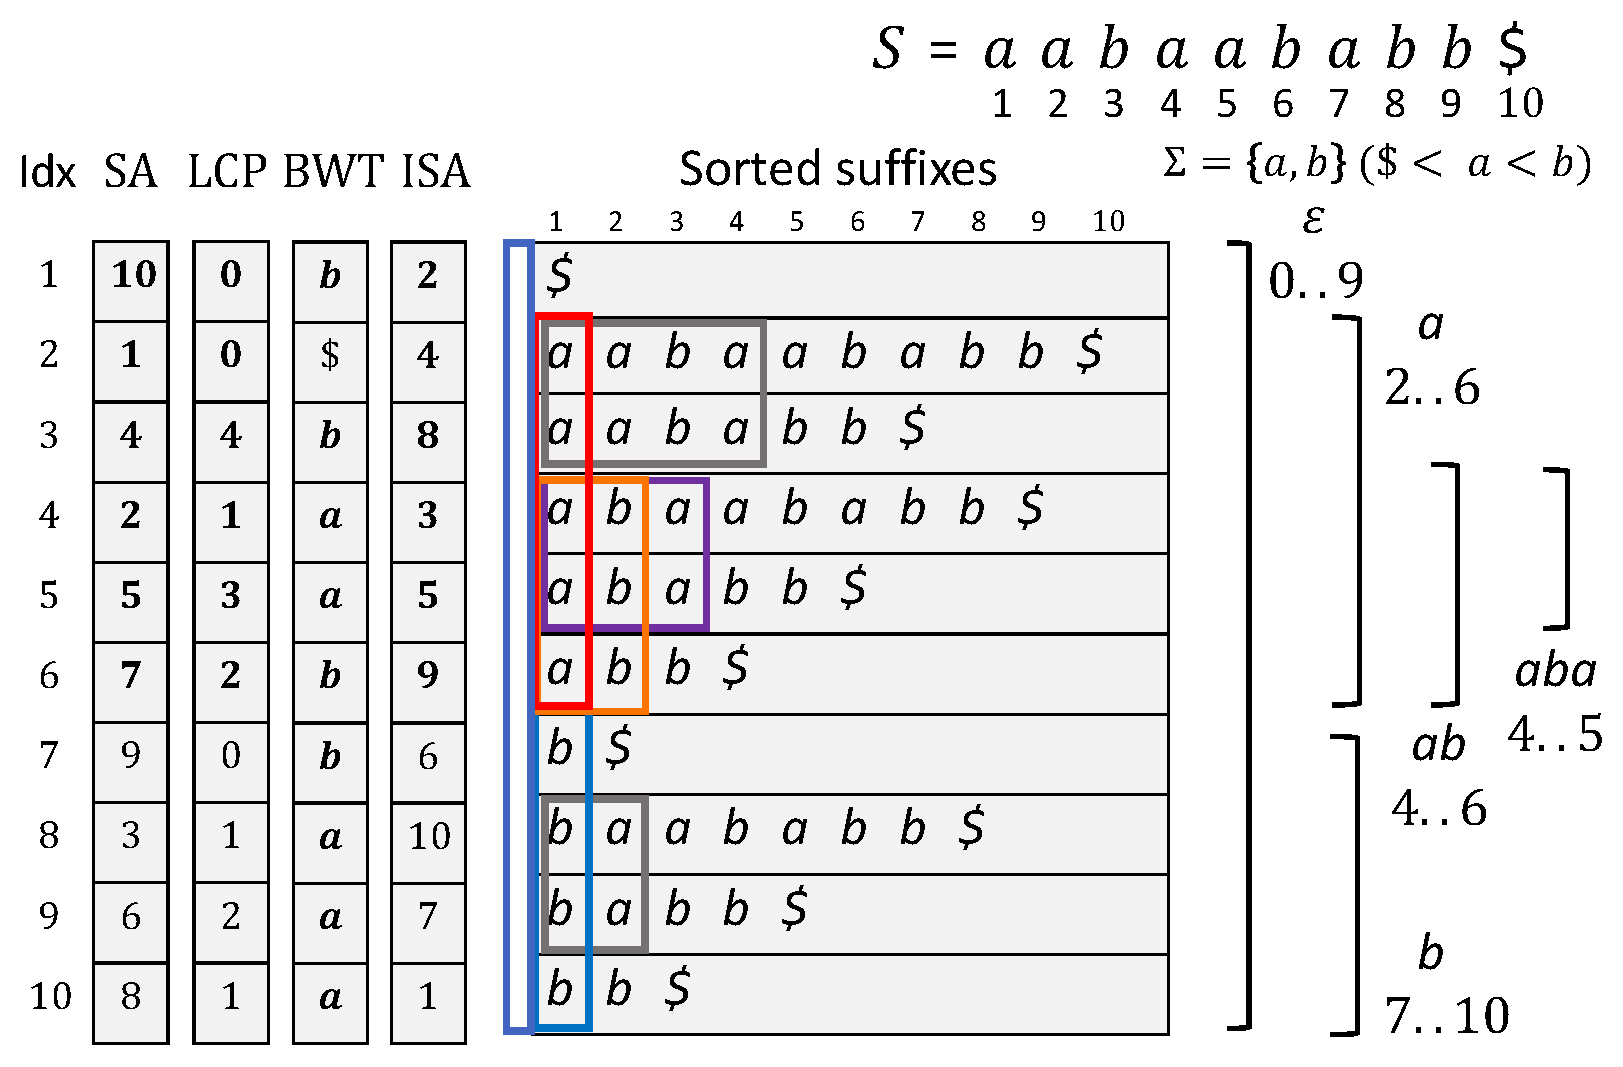
\includegraphics[height=0.39\textwidth]{fig1.pdf}
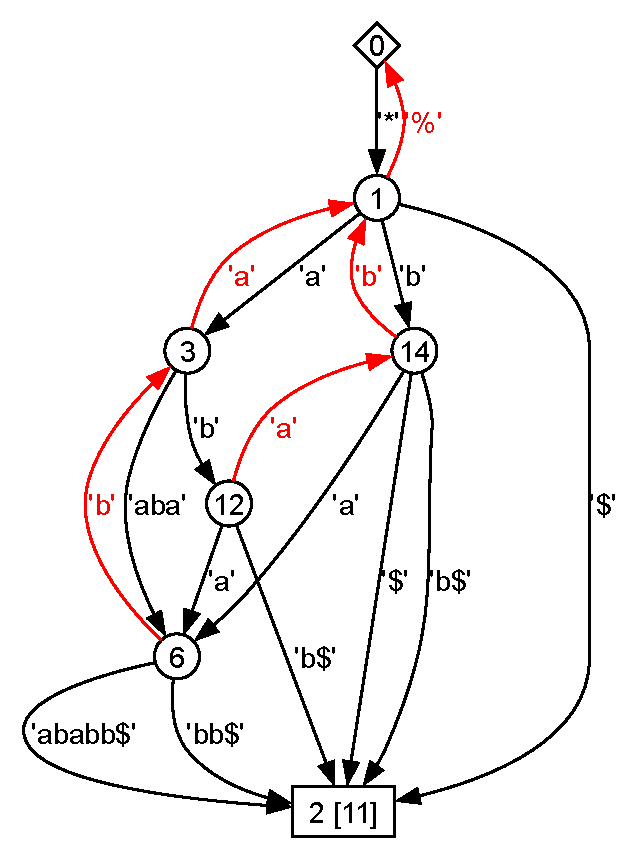
\includegraphics[height=0.39\textwidth]{fig7.pdf}
\vspace{.5\baselineskip}
\caption{An example of indexing arrays $SA, LCP, BWT, ISA$ of a string $S$ as an input (left) and its CDAWG $G$ as an output (right),
where a string is $S[1..10] = aabaababb\daller$ of length $n = 10$ over alphabet $\Sigma = \set{a, b}$ and its index starts at $0$. 
  In $S$, the left endmarker $S[0]=\#$ and the related suffixes are omitted. In $G$, nodes $0$ and $1$ indicate a virtual master node and the root, respectively. Black and red arrows indicates the goto edges and suffix links, respectively. 
  We observe that branching nodes $1, 3,14,12$, and $6$ of $G$ correspond to maximal repeats of $S$, namely, $\eps$, $a$, $b$, $ab$, and $aaba$. 
%%   Inside and to the right of the panel for sorted suffixes, each bold rectangle $R = [i..j]\times [0..\ell-1]$ and square bracket
%% indicate a rich representation $(i..j, \ell)$ of a repeat of $S$ and 
%% the associated SA-interval $i..j$, respectively. 
}\label{fig:example:arrays}
\end{figure}
%%%%%%

%% %%%% 
%% \section{Notes}
%% \label{sec:notes}




\section{Outline of the Proposed Algoritm}
%\section{Top-level Structure of Algoritm}
%%%% 

In this section, we present an $O(e_{\max})$-expected time solution over an integer alphabet.
%% \subsection{Outline of the algorithm}
%% %%%
Let $\Sigma$ be an alphabet with $|\Sigma(S)| \ge 2$ characters. 

%% \subsection{The recursive procedure $\RecLPT$}
\subsection{Top-level structure of algorithm}
%%%%
In \cref{algo:main}, we show the top-level structure of our algorithm for transforming the suffix array of a string $S$ with auxiliary structures with length $n$ into the CDAWG $G$ of the string as follows, where $\pair{1..n, 0}$ indicates the root of the CDAWG to be constructed in a representation introduced later in \cref{sec:constant:size:rep}. 
%%%%
{
% \setlength{\interspacetitleruled}{0pt}%
\setlength{\algotitleheightrule}{0pt}%
\begin{algorithm}[h]
  \caption{Transforming $SA$ and $S$ into its CDAWG $G$.
    %% Transforming the suffix array of a string $S$ with auxiliary structures with length $n$ into the CDAWG $G$ of the string.
  }\label{algo:main}
\KwPreproc{Construct an index $\sig I = (\SA, \ISA, \LCP)$ from $SA$ and $S$.}  
\KwRuntime{Perform the following steps on request}
\Begin{
    $T \gets \RecLPT(\pair{1..n, 0}, \sig I, S)$
      \Comment*{Compute $\LPT(S)$ from $\sig I$}
    $G \gets \RecCDAWG(T, S)$
      \Comment*{Compute $\CDAWG(S)$ from the $\LPT(S)$} \label{line:main:merge}
      %%  obtained from $\LPT(S)$ by merging non-maximal nodes to maximal nodes
    Return $G$\; 
}
\end{algorithm}
}
%%%%%%%%%

In preprocessing, an index structure $\sig I = (\SA, \ISA, \LCP, S)$ is constructed from an input string~$S$ of length $n$ over $\Sigma$ in linear time using appropriate construction algorithms~\cite{navarro2016cds:book,navarro2021indexing:ii}.
In runtime, the CDAWG $G$ of $S$ is constructed on $\sig I$ through construction an intermediate structure $\LPT(S)$, called the extended longest common prefix tree of $S$.

In an application senario in a human genome repository, the structure $\sig I$ will be constructed once, reside on memory using $O(n)$ space, and be used many times for the generation of the CDAWG in $O(e_{\max})$ time and working space per execution, and other purposes, such as the standard string search.
To describe our algorithm, we introduce a virtual rooted tree $\LPT(S)$ as follows according to \cite{belazzougui:nunial:gagie:prezza:raffinot2015composite,inenaga2024computing}. 

\begin{definition}[informal]\rm 
The \textit{extended longest common prefix tree} (or the \LPTrm-tree) of a string $S$, denoted $\LPT(S) = (\sig V, \sig E, \eps)$, is an edge-compacted rooted tree obtained from the CDAWG $G = (V(G), E(G), \eps)$ of $S$ by cutting all non-primary arcs in $E(G)$ to separate them from maximal repeats, and replacing their targets with newly created nodes.
$\sig V = V(G)\uplus\Delta(S)$ is a node set,%
%%
\footnote{Belazzougui~\textit{et al.}~\cite{belazzougui:nunial:gagie:prezza:raffinot2015composite} introduced the \LPTrm-tree of $S$ to show that the parameters $r(S)$ and $z(S)$ are upperbounded by $O(e_R(S) + e_L(S))$, where the set $\V(G)$ and $\Delta(S)$ are written as $\sig E$ and $\sig F$, and each element of $\sig F$ is called a \textit{fringe}. Inenaga et al.~\cite{inenaga2024computing} used \LPTrm-tree to compute all distinct minimal absent words of a string $S$ in output linear time. 
}
%%
where the set $V(G)$ correspoind to all maximal repeats and $\Delta(S)$ corresponds to all new nodes representing non-maximal repeats.
\end{definition}

  $\LPT(S)$ can be stored in $O(e_R)$ words, and can be easily converted into the CDAWG $G$ in $O(e_R)$ time.

\subsection{Constant-size Representation of factors}
\label{sec:constant:size:rep}
%%% 
%% We encode any factor, including maximal repeats, of $S$ in a constant-sized representation as follows so that it can be operated in constant time.
We introduce a representation of any factor of $S$ in constant space so that it can be manupilated in constant time. 
The \textit{rich representation} of a factor $u$ of $S$ is a triple $\tau = (i, j, \ell) \in [n]^3$, denoted by $\pair{i..j, \ell}$, consisting of 
\begin{itemize}
\item the pair $(i, j)$ with $1\le i\le j\le n$ represents the \textit{SA-range} $i..j\subseteq 1..n$ of $u$ that is the maximal range
  %% w.r.t.~set-inclusion
  consisting of all suffixes of $S$ prefixed by $u$, and  
  
\item the integer $\ell\ge 0$ represents the length of the factor $u$, namely, $\ell = |u|$. 
\end{itemize}

We denote by $\RR$ the set of the rich-representation of all factors of $S$.
We used the constant-sized representation of factors of $S$ \cref{sec:sa:to:lpt} in the followings. 


%%%%%%%%%%%%%%%%
\section{Transforming Suffix Array to \LPTrm-tree}
\label{sec:sa:to:lpt}

In this section, we present the first algorithm $\RecLPT$ for transforming the suffix array for a string $S$ into its \LPTrm-tree used at \cref{line:main:merge} in \cref{algo:main}.


\subsection{Outline}
%% \subsection{Recursive subprocedure}
%%%% 
In \cref{algo:rec}, we show the recursive subprocedure $\RecLPT$ that given the triple $\pair{1..n, 0}$ for the empty string $\eps$, recursively constructs the extended LPT tree $T = \LPT(S)$ of a string $S$ on an index structure~$\sig I$. It systematically enumerates the set $\MR(S)$ of all maximal repeats, a class of special factors of $S$, in top-down manner from shorter to longer. In the procedure $\RecLPT$, each maximal repeat $u$ is encoded as the triple $\pair{i, j, \ell} = \pair{i..j, \ell}$, called the rich-representation, or simply the \textit{triple} of $u$, where $i..j$ is its SA-range of $u$ in $SA$ and $\ell = |u|$ is its length.

The procedure $\RecLPT$ works as follows: 
%%where maximal repeats are a class of special factors of $S$. 
\begin{itemize}
\item It starts with the triple $\op{rep}(\eps)$ of the shortest maximal repeat, i.e., $\eps$, and the initial DAG $G = (\set{\eps}, \emptyset{}, \eps)$. 
  
\item At each iteration with the triple $\op{rep}(u) = \pair{i..j, \ell}$ of a maximal repeat $u \in \MR(S)$, it generates the triples of a maximal repeat $v_b$ in $\MR(S)\setminus{\eps}$ as a children of $u$ for possible character $b\in\Sigma$, and then, recursively call itself with $v$ and $G$ as arguments. The generation of children of the parent $u$ will be described in the later subsections. 
\end{itemize}

To show the correctness and time complexity, we will show that $\RecLPT$ simulate a top-down traversal of $\LPT(S)$ by visiting all of $O(\mu(S))$ members of $\MR(S)$, following $O(e_R(S))$ arcs, and backtracking when it eventually reaches a non-member of $\MR(S)$.
In the following subsections, we will explain more details of the above procedure. 

%% The tree $\LPT(S)$ is rooted at the empty string $\eps$ as the shortest maximal repeat, and whose edge set $\sig E = \sig E \cup \sig F$ consists of the set $\sig E$ of all edges connecting maximal repeats, and additionally contains a set $\sig F$ of edges that are associated with the failure of traversal. 

\subsection{Enumeraton of maximal repeats of $S$}  
%%\subsection{The $\LPT(S)$ tree}
%%% 
The tentative goal here is to generate all maximal repeats without duplicates in amortized constant time per solusion. For the purpose, we introduce the LPT tree of $S$, $\LPT(S)$, which will be shown to be a subgraph of the suffix tree of $S$ later. Then, we give a high-level description of our algorithm.

\subsubsection{Relationship between $\Stree(S)$ and $\CDAWG(S)$}
%%%
Consider the suffix tree $\Stree(S) = (V, E, \underline\eps)$ of a string $S$. 
%% Recall that $\underline u$ is the locus of a factor $u$ such that $\str(\underline u) = u$. 
In $\Stree(S)$, we observe that all branching nodes correspond the loci $\underline u$ of all right-branching factors $u$ of $S$, while all leaves correspond to the loci $\underline s$ of all suffixes $s$ of $S$.

\begin{remark}\label{remark:one:primary}
  For any factor $u \in \Sigma^*$ of $S$, the conditions (1)--(3) are equivalent:
  \begin{enumerate}[(1)]
  \item The locus $\underline{u}$ of $u$ in the CDAWG of $S$ is a branching node and $u$ is the string label of the longest path from the source to $\underline{u}$. 
  \item The locus $\underline{u}$ of $u$ in the suffix tree of $S$ is a branching node and has two or more incoming suffix links. 
  \item The string label $u$ is a maximal repeat of $S$, i.e., $u \in \MR(S)$. 
  \end{enumerate}
\end{remark}


%%%%%%%%%%%%%5
\begin{algorithm}[t]
  \caption{
    A subprocedure $\RecLPT$ for constructing the extended LPT-tree $\LPT(S)$ of the string $S$ on an index $\sig I = (\SA, \ISA, \LCP, S)$.
    %% for enumerating the set $\MR(S)$ of all maximal reepeats of the string $S$ prefixed by the word $u := \getfactor(i..j, \ell)$. 
}\label{algo:rec}
%%%\medskip
  \KwInput{
    A triple $\pi = \pair{i..j, \ell} \in \RR$ and a rooted tree $T = (\sig V(T), \sig E(T), \eps)$. 
  }
  \KwOutput{
    A subgraph $T = (\sig V(T), \sig E(T), \eps)$ of $\LPT(S)$. 
  }
  \textbf{procedure} \RecLPT$(\pi, T)$\;
  \Begin{
      \Comment{Pre-condition: $\pi = \pair{i..j, \ell}$ represents a maximal repeat $u$ in $\MR(S)$.}
      %% $Children \gets \emptyset$\; 
      $Children \gets \GenChildren(i..j, \ell, \op{undef})$\Comment*{See \cref{lem:genchildren}}
      \label{line:recmr:for:begin}
      \For {each child $(c, \tau_c = \pair{i_c..j_c, \ell_c})$ in $Children$}{
             \Comment{Post-condition:
               $c \in \RChar(u)$ is a branching character and 
               $\tau_c$ represents
               an $c$-child $\rext{uc} \in \MR(S)$ of $u$. 
             }
             $\sig V(T) \gets \sig V(T) \cup\set{ \tau_c }$
             \Comment*{Adding a node to $\sig V(T) = \MR(S)\cup\Delta(S)$}
             $\sig E(T) \gets \sig E(T) \cup\set{ (\pi, \tau_c) }$
             \Comment*{Adding an arc to $\sig E(T) = \sig E\cup\sig F$}
             \uIf (\comblk{See \cref{lem:leftmaximal:character}}) {$\isLeftBranching(i_c..j_c, \ell_c)$}{
               $\RecLPT(\tau_c, T)$
               \Comment*{A node $\tau_c \in \sig M$ for a maximal repeat}
               \label{line:recmr:for:end}
             } %% If
             \Else{
               $\rhd$ do not recurse
               \Comment*{A dammy leaf $\tau_c \in \Delta$ and $(\pi, \tau_c) \in \sig F$, resp.}
             } %% Else
       } %% for 
    }
\end{algorithm}
%%%%%%%%%%%%%%%%%



We need a few technical definitions. 
For any factor $u \in \Sub(S)$, we define the \textit{right-closure} of $u$, denoted $\rext{u}$, to be the string obtained from $u$ by maximally extending $u$ rightwards while the occurrence of the resulting substring does not change, i.e., $\Spos(\rext{u}) = \Spos(u)$ holds.
Similarly, we can define the \textit{left-closure} of $u$, denoted $\lext{u}$ by symmetry. 
%%
For example, consider a string  $S[1..n] = \mathtt{aabaababb\$}$ of length $10$. For a factor $aa$ with $\Spos(aa) = \set{1, 4}$, its right-closure is $\rext{aa} = aaba$. On the other hand, for a factor $a$ with $\Spos(a) = \set{1,2,4,5,7}$, its right-closure is $\rext{a} = a$. 

%% %%This definition is well-defined since the longest path is closed under prefix.
%% Next, in the suffix tree $T$ of $S$, with a slight abuse of terminology, a (unique) path $\pi$ from the root to a node $\underline v$ is said to be \textit{primary} if its corresponding path in $G$ is primary. Again, a primary path is closed under prefix. Then, any arc $f = (\underline u, \underline v)$ in $T$ is said to be \textit{primary} if it is included in a primary path $\pi$ to $\underline v$, and \textit{non-primary} otherwise. 

%% From the equivalence shown in \cref{remark:one:primary}, we introduce the primary arcs in the CDAWG $G$ and suffix tree $T$ of $S$. In $G = \CDAWG(S)$,  any arc $f = (\underline u, \underline v)$ is said to be \textit{primary} if it is included in the longest path from the root to node $\underline v$, and \textit{non-primary} (or secondary) otherwise.
%% %%This definition is well-defined since the longest path is closed under prefix.
%% Next, in the suffix tree $T$ of $S$, with a slight abuse of terminology, a (unique) path $\pi$ from the root to a node $\underline v$ is said to be \textit{primary} if its corresponding path in $G$ is primary. Again, a primary path is closed under prefix. Then, any arc $f = (\underline u, \underline v)$ in $T$ is said to be \textit{primary} if it is included in a primary path $\pi$ to $\underline v$, and \textit{non-primary} otherwise. 

\subsubsection{The extended longest common prefix tree of $S$}
%%%
We introduce subgraphs $\LPT(S)$ and $\LPT(S)$ of $\Stree(S)$ in the followings. First, we define the subsets of nodes $\sig V(S), \Delta(S) \subseteq V$ and the subsets  of arcs $\sig E(S), \Delta(S)\subseteq E$ as follows: 
\begin{itemize}
\item $\sig V$ is the subset of the nodes corresponding to all maximal repeats, that is, $\sig V = \set{ \underline u \mid u \in \MR(S) }$. 
  
\item $\sig E \subseteq E$ is the subset of all arcs $f = (u, v)$ in $E$ that connect maximal repeats in $\MR(S)$, that is, $\sig E = \sete{ (\underline u, \underline v) \in E \mid \set{u, v} \subseteq \MR(S) }$.

\item $\sig F\subseteq E$ is the subset of all arcs $f = (u, v)$ in $E$ that connect a maximal repeat $u$ and a non-maximal repeat $v$, that is, $\sig F = \sete{ (\underline u, \underline v) \in E \mid u \in \MR(S), v \not\in \MR(S) }$.  
%% $\sig E(S) = \sig E(S) \cup \sig F(S)$ is the subset of $E$, where
  
\item $\Delta(S) = \set{ \underline v \mid f = (\underline u, \underline v) \in \sig F }$ is the set of the destinations of all arcs in $\sig F$.
%% $\sig V(S) = \sig V(S) \cup \Delta(S)$ is the subset of $V$, where 
\end{itemize}

By construction,
%% it follows that $\sig V(S)\subseteq \sig V(S) \subseteq V(S)$ and $\sig E(S)\subseteq \sig E(S) \subseteq E(S)$. Moreover,
$\sig V(S)$ contains the shortest maximal repeat $\eps$. The DAG $\LPT(S)$ is called the longest common prefix tree of $S$ in the literature.  

\begin{definition}[Belazzougui \textit{et al.}~\cite{belazzougui:nunial:gagie:prezza:raffinot2015composite}, Inenaga \textit{et al.}~\cite{inenaga:iwoca2024computing:maw}]
  We define the extended longest common prefix tree of $S$ to be the rooted DAG $\LPT(S) = (\sig V(S), \sig E(S), \eps)$, where 
  $\sig V(S) = \sig V(S) \cup \Delta(S) \subseteq V$ is the node set, $\sig E(S) = \sig E(S) \cup \sig F(S) \subseteq E$ is the arc set, and $\eps \in \sig V(S)$ is the root. 
\end{definition}

Blumer \textit{et al.}~\cite{blumer1987complete} showed the properties of the CDAWG $G$ of $S$, which is the minimum state DFA of $\Suf(S)$ with path-compression. We define the \textit{end-equivalence relation} $\equiv_{epos}$ over $\Sub(S)$ by $x \equiv_{epos} y \iff\Epos(x) = \Epos(y)$.
%%%
Each node $\underline u$ of $G$ with $u \in \Sub(S)$ represents an equivalence class, denoted by $[\rext{u}]^S_{epos} \subseteq \Sub(S)$, of factors of $S$ with respect to $\equiv^S_{epos}$. That is, $\underline u := [\rext{u}]^S_{epos} = \sete{ v \in \Sub(S) \mid u \equiv_{epos} v}$.
%% Then, each node $\underline u$ of $G$ represents the equivalence class $[\rext{u}]^S_{epos} \subseteq \Sub(S)$ of factors of $S$ with a representative $u \in \Sub(S)$ w.r.t.~$\equiv^S_{epos}$, namely, $\underline u := [\rext{u}]^S_{epos} = \sete{ v \in \Sub(S) \mid u \equiv_{epos} v}$.
%%%
%% Usually, the longest element, denoted by $\Value(\underline u)$ is used as the representative of $\underline u = [\rext{u}]^S_{epos}$.
The representative of $\underline u = [\rext{u}]^S_{epos}$ is the longest element, which we denote by $\Value(\underline u)$. 
Each member $v$ of the equivalence class $[\rext{u}]^S_{epos}$ is the string label of a path from the root to node $\underline u$. 
All arcs in the CDAWG $G$ can be classified as either primary or non-primary. An arc $f = (\underline u, \underline v)$ is said to be \textit{primary} if it is included in the longest path from the root to node $\underline v$, and \textit{non-primary} (or secondary) otherwise.
Note that only a subset of arcs of $\Stree(S)$ can be included in $\CDAWG(S)$ in general. 

\begin{lemma}[Belazzougui \textit{et al.}~\cite{belazzougui:nunial:gagie:prezza:raffinot2015composite}]\label{lem:lpt:edge:classification}
  The arc subsets $\sig E$ and $\sig F$ of $\LPT$ correspond to the sets of all primary arcs and all non-primary arcs in $G = \CDAWG(S)$. That is, for all pair of factors $u, v\in \Sub(S)$, the arc $f = (\underline u, \underline v)$ in $\sig E$ and the corresponding arc $f' = ([\rext{u}]^S_L, [\rext{v}]^S_L)$ satisfies the conditions (1) and (2) below: 
\begin{enumerate}[(1)]  
\item $f \in \sig E\cup \sig F$ if and only if $f$ is an arc of $G$. 
\item Moreover, (i) $f \in \sig E$ if and only if $f'$ is a primary arc of $G$, while (ii) $f \in \sig F$ if and only if $f'$ is a non-primary arc of $G$.
\end{enumerate}
\end{lemma}

%% \begin{proof} TBD. 
%% \end{proof}

From \cref{lem:lpt:edge:classification}, we refer to the arcs $f$ of $\LPT(S)$ as \textit{primary} if $f \in \sig E$ and as \textit{non-primary} if $f \in \sig F$ without confusion. Then, we can identify $\LPT(S)$ and $G = \CDAWG(S)$, where we can obtain the former from the latter by replacing each secondary arc $f = (\underline u, \underline v)$ by a new arc $f' = (\underline u, \underline {v_f})$ with a new end point $\underline{v_f}$ and the associated string label $v_f = \Value(\underline u)\cdot \lab(f) \in \Sigma^+$. 

\subsection{Simulating a traversal of $\LPT(S)$}
%%%%
Since the node set of $\LPT(S)$ equals the set $\MR(S)$ as its nodes, we can enumerate all maximal repeats in $\MR(S)$ by a top-down traversal of $\LPT(S)$ using backtracking starting from the representation $\tau_\eps \in \RR$ for the root $\eps$, and expanding the current representation $\tau \in \RR$ for a maximal repeat $u \in \MR(S)$ into the set of its children $Children(\tau) \subseteq \RR$.
Below, we will inductively construct a spanning tree over the set $\MR(S)$ by induction on the length of a string as follows.

In the base case, we can easily see that the empty string $\eps$ is the shortest member of $\MR(S)$ due to the assumption $|\Sigma|\ge 2$. Then, it is easy to see that the triple for $\eps$ is given by $\pair{1..n, 0}$. 

In the induction case, we try to generate the triple for a maximal repeat $v\in \MR(S)$ from the triple for a shorter maximal repeat $u\in \MR(S)$.
%% Then, the parent $u$ of a maximal repeat $v \in \MR(S)$ is the maximal repeat $u \in \MR(S)$ such that
For any arc $f = (\underline u, \underline v) \in \E\cup\F$ in $\LPT(S)$, we say that $u$ is the \textit{parent} of $v$, and $v$ is a \textit{child} of $u$. 
Generation of the set $Children(\tau)$ can be done as follows.

%% Note that a factor $v$ of $S$ is left-branching only if its SA-range $i..j$ have width two or more, i.e., $|i..j| \ge 2$. 

\begin{lemma}\label{lem:maxrep:howto:child}
  Let $\LPT(S) = (\sig V, \sig E, \eps)$
  For any maximal repeat $u \in \Sigma^*$ in $\MR(S)$ and any non-empty string $v \in \Sigma^+$, the following conditions (1) and (2) are equivalent: 
\begin{enumerate*}[(1)]
\item $v \in \sig V$ and $u$ is the parent of $v$;  
\item
  \begin{enumerate*}[(i)]
  \item $v = \rext{(ua)}$ for a character $a\in \Sigma$, and 
  \item $v$ is a left-branching factor of $S$. 
    %% \item $|i..j| \ge 2$ with
    %% the SA-range $i..j$ of $v$. 
  \end{enumerate*}
\end{enumerate*}
\end{lemma}

%%%%%%%%%%%%%%%%%%%
{
%% \setlength{\interspacetitleruled}{0pt}%
\setlength{\algotitleheightrule}{0pt}%
\begin{algorithm}[h]
  \caption{
    \textbf{Procedure} $\GenChildren(\pair{i..j, \ell_*}, Children)$.  
  }\label{algo:genchildren}
  %% \KwInput{the triple $W = (i..j, \ell_*)$ for a factor of $S$.}
  %% \textbf{Procedure} $\GenChildren(\pair{i..j, \ell_*}, Children)$:\\
  \Comment{\textit{Notes}: $S$ and $SA$ at \cref{line:genchildren:compute:ch} are only for explanation, and can be omitted.
  }
  %% \Begin{
      \If  (\comblk{
        $|i..j| = j - i + 1$.
        %% $\pair{i..j, \ell}$ has no unique occurrences
      })
           {$|i..j| \ge 2$}
           %% {$j - i + 1 \ge 2$}
      {
        $(m, \ell_m) \gets RMQ_{LCP}(i+1, j)$
        \Comment*{$\ell_m = LCP[m]$}
        \uIf (\comblk{$i..j$ is monotone}) {$\ell_* < \ell_m$}{
          %% $p \gets SA[i]$\;
          $ch \gets S[SA[i]+\ell_*]$
          \Comment*{Notes: $ch$ is used for explanation only}
          \label{line:genchildren:compute:ch}
          $Children.\append(\pair{ch, \pair{i..j, \ell_m}})$
          \Comment*{A child $\pair{ch, \pair{i..j, \ell_m}}$}
        }
        \Else  (\CM{$\ell_* = \ell_m$} and $[i,j]$ is diverse) 
        {
          $\GenChildren(\pair{i..m-1, \ell_*}, Children)$\; 
          $\GenChildren(\pair{m..j, \ell_*}, Children)$\;
        }
      }
      \Return $Children$\;
  %% } %% Begin
\end{algorithm}
}
%%%%%%%%%%%%%%%%%

\subsection{Generation of the set of child triples}
%%%% 
An SA-range $i..j$ is called an \textit{$\ell$-range} if the lcp of all suffixes starting  with positions in $SAi..j$ equals~$\ell$, i.e.,
\begin{align}
  \ell
  &= lcp(\set{ S[p..n] \mid p = SA[k], k \in i..j } ) 
\\&= \min\sete{ LCP[k] \mid k \in [L+1..R] },   
\end{align}
where $LCP[k] = lcp(S[p..n], SA[q..n]])$ with $p = SA[k]$ and $q = SA[k-1]$. 
Then, an index $k \in i+1..j$ such that $LCP[k] = \ell$ is called a \textit{$\ell$-index}. 
Cosider the suffix tree $\sig T$ of a string $S$.
%% We say that a triple $\tau = (i..j, \ell)$ is a child of triple $\tau_0 = ([L_0..R_0], \ell_0)$
For two triples $\tau_i$ for factors $u_i$ for every $i = 1,2$, we say that $\tau_1$ is the parent (resp.~a child) of $\tau_2$ if and only if $u_1$ is the parent (resp.~a child) of $u_2$.

We remark that any SA-range $i..j$ without a length component $\ell$ implicitly represents a right-maximal factor of $S$. More precisely, we observe that a triple $\pi = \pair{i..j, \ell}$ represents a right-maximal factor of $S$ if and only if $i..j$ is an $\ell$-range. We always assume that a parent $\pi$ satisfies this condition. 
For generating the set $Children(\tau)$ of all child triples of a given parent tripel $\tau$, we use the following lemma, shown by . Abouelhoda, Kurtz, and Ohlebusch~\cite{abouelhoda2004replacing}. 

\begin{lemma}[Abouelhoda \textit{et al.}~\cite{abouelhoda2004replacing}]\label{lem:child:ranges}
  Let $\pi = [i_0..j_0]$ be any $\ell$-range.
  If $m_1 < m_2 < \dots < m_k$ are the $\ell$-indexes in ascending order, then the child ranges of $\pi$ are
  $[i_0..m_1-1], 
   [m_1..m_2-1], 
   \ldots,
   [m_k..j_0]$.  
\end{lemma}

Abouelhoda \textit{et al.}~\cite{abouelhoda2004replacing} presented an algorithm for generating all child triples using an extra array $\op{childtab}[1..n]$ of cells with three integer fields $\op{up}, \op{down}$, $\op{nextIndex} \in [n]$ in addition to $\SA$ and $\LCP$. 
%%However, the method is not suitable to our purpose. 
%%% 
Instead of the $\op{childtab}$ array, we present another method using $\SA$ and the RMQ structure on $\LCP$ (denoted $RMQ_{\LCP}$) as follows.%
%%%% 
\myfootnote{We remark that the string $S$ in $\GenChildren$ can be omitted since it is used to get right-brancing characters, only for explanation, and not used by $\RecLPT$ of \cref{algo:rec}. }
%%%% 
%% generate the set $Children(\pi)$ of all child triples of a parent triple $\pi$. 
As a key component,
we use the implementation of the colored range query
based on \cref{lem:child:ranges}, proposeby Muthukrishnan~\cite{muthukrishnan2002efficient} (see also the textbook by Ohlebusch~\cite{ohlebusch2013bookbioinfo}).

\begin{lemma}[Muthukrishnan~\cite{muthukrishnan2002efficient} and Ohlebusch~\cite{ohlebusch2013bookbioinfo}]\label{lem:genchildren}
  The set of all child ranges of an $\ell$-range $i..j$ can be enumerated in $O(occ)$ time in $O(\sigma)$ working space
  using the $RMQ_{LCP}$ structure of $O(n)$ words, 
where $occ$ is the number of the child renges to output.  
\end{lemma}

Based on \cref{lem:genchildren}, \cref{algo:genchildren} presents the procedure $\GenChildren$, which recusively generates the set of child triples
\begin{align}
  Children(\pi)
  &= \sete{ (c, \tau_c) \mid c \in \LChar(u), \tau_c = \pair{i..j, \ell} \in Children(\pi)}, 
\end{align}
invoked with a parent triple $\pi = \pair{i..j, \ell_*}$ with $\ell_*$-range for a maximal repeat $u$ and the pointer $Children$ to the empty set $\emptyset$,
where $\tau_c$ is the triple for a maximal repeat $\rext{(uc)}$ with a branching character $c \in \LChar(u)$.

\subsection{Efficient test of the left-brancing condition}
%%% 

Recall that a repeat is maximal if and only if it is both left- and right-maximal in $S$. Since the node set $\sig V+$ of $\LPT(S)$ is closed under taking parents, we have the next lemma.

\begin{lemma}\label{lem:prune:leftbranch}
Suppose that a triple $\pi$ is an ancestor of a triple $\tau$. If the substring $ub$ defined by $\tau$ is left-branching, the substring $u$ defined by $\pi$ is also left-branching. 
\end{lemma}

\begin{proof}
  For any $v = ub$ with some $b \in \Sigma$, we can show that
  $\LChar(ub) \subseteq \LChar(u)$, and thus that $|\LChar(ub)| \le |\LChar(u)|$. On the other hand $ub$ is right-brancing in $S$ if and only if $2\le |\LChar(ub)|$. It immediately follows that $2 \le |\LChar(u)|$ meaning that $u$ is right-brancing in $S$. This shows the lemma. 
\end{proof}


Since the nodes of the set $\sig V$ represents all and only the right-branching factors, \cref{lem:prune:leftbranch} implies the next rule.

\begin{itemize}\item[]
\quad\textsc{Pruning rule}: {Every non-left-branching triple is pruned.}
\end{itemize}

We explain how to efficiently test whether a given triple $\tau = \pair{i..j, \ell}$ represents a left-branching factor of $S$. For this purpose, we use the following lemma, which is a slight modification of Narisawa \textit{et al.}~\cite[Lemma~10]{narisawa2007efficient}.

\begin{minipage}{\textwidth}
\begin{lemmarep}[Narisawa \textit{et al.}~\cite{narisawa2007efficient}]\label{lem:leftmaximal:character}
  For the triple $\tau = (i..j, \ell)$ for any substring~$u$ of $S$,
  \begin{enumerate}[(1)]
\item $u$ is not left-branching in $S$ if and only if  
\item (i) $S[p-1] = S[q-1]$ and (ii) $j - i = \id{ISA}[p-1] - \id{ISA}[q-1]$, 
\end{enumerate}
where $p = SA[i]$ and $q = SA[j]$.
\end{lemmarep}
\end{minipage}
\medskip 

\begin{proof}
%%We add clause (*)  
We let $p = SA[i], q = SA[j]$. 
$(1)\Implies (2)$: Suppose that $u$ is not left-branching in $S$.
Then, all occurrences of $u$ in $S$ have the same previous characters $c \in \Sigma$ in $\Spos(u)$. Thus, it immediately follows that $BWT[i..j]$ is monotone.
Let $\varphi: k \mapsto ISA[SA[k]-1]$. By observing $\varphi$ coincodes to the LF-mapping~\cite{Ferragina05:FM}, claim (2) immediately follows. 
%%% 
$(2) \Implies (1)$: 
Suppose (2), and to contradict that $\neg$(2) $u$ is left-branching in $S$. Let $I = i..j$. Then, there exist a pair of preceding characters $c = S[p-1], d=S[q-1]$ with $c\not= d$ for some $p, q \in \Spos(u)$. It follows that $\varphi$ transforms the positions in  $SA[i..j]$ into at least two, mutually disjoint, non-empty ranges $I_c, I_d$ with $I_c\uplus I_d = I$ starting with $c$ and $d$, respectively. By assumption (2.i), we see that positions $SA[i]$ and $SA[j]$ move into the same range, say $I_c$ with $i_c := \varphi(i)$ and $j_c := \varphi(j)$ as the left and right ends of $I_c$ since $\varphi$ preserves $<_\lex$. 
Since both of $I_c$ and $I_d$ are non-empty, we have $j_c - i_c + 1 = |I_c| < |I| = j - i + 1$; contradiction to assumption (2.ii). By contradiction, we conclude condition (1) holds. 
%% \qed   
\end{proof}

From \cref{lem:leftmaximal:character}, we can implement the procedure $\isLeftBranching(i..j, \ell)$ for testing the left-branching property of a triple $\tau = \pair{i..j, \ell}$. The code for $\isLeftBranching$ is omitted. 



\subsection{Analysis}

We show the correctness and computational complexity of the procedure $\RecLPT$ in \cref{algo:rec:cdawg} as follows. 

\begin{lemmarep}[correctness and time complexity]\label{lem:main:from:lpt:to:cdawg:correct:time}
  Let $T$ be the $\LPT(S)$ of a string $S$ of length $n$. 
  The procedure $\RecLPT$ in \cref{algo:rec:cdawg} computes $T = \LPT(S)$ from the static index $\sig I = (\SA, \ISA, LCP)$ and the read-only copy of $S$
  in $O(e_R(S) + e_L(S))$ time using $O(\max\{e_R(S), e_L(S), \sigma\log n\})$ space. 
\end{lemmarep}

\begin{proofsketch}
  From
\cref{lem:maxrep:howto:child},
\cref{lem:genchildren},
\cref{lem:leftmaximal:character},
and the construction of $\LPT(S)$,
the correctness of the recursive procedure $\RecLPT$ follows.
For the time complexity, we observe that the algorithm traverses each arc and nodes exactly once from \cref{lem:maxrep:howto:child}. Since at each iteration, $\GenChildren$ and $\isLeftBranching$ require at most $O(e_R)$ total time, the algorithm runs in $O(e_R(S))$ total time. Space use of all components other than the stack usage is $O(\sigma)$. To bound the usage of the call stack of $\RecLPT$, we can apply the heavy path decomposition of the suffix tree by Belazzougui \textit{et al.}~\cite{belazzougui2020linear} to obtain $O(\sigma \log n)$ memory usage for the stack. This completes the proof. 
\end{proofsketch}

\begin{proof}
From
\cref{lem:maxrep:howto:child},
\cref{lem:genchildren},
\cref{lem:leftmaximal:character},
and the construction of $\LPT(S)$, 
the recursive procedure $\RecLPT$ in \cref{algo:rec} correctly construct all nodes and edges of $\LPT(S) = (\sig V(S), \sig E(S), \eps)$ by generating all maximal repeats by starting with the root $\eps$, and by following all arcs $(u, v)$ in $\E(S)$ defined with the right-closure $v = \rext{(ub)}$ of a right-extension $ub$ with a branching character $b$ using a depth-first traversal of $\LPT(S)$.
From \cref{lem:prune:leftbranch}, we see that if it eventually reaches a non-maximal node in $\Delta(S)$, it correctly stops the search and backtracks. Each arc is added to the arc set whenever it is traversed. Since each node $\underline v$ in $\E(S)\cup \F(S)$ can be reached through exactly one incoming arc, the procedure correctly find all arcs.
For the time complexity, it follows from \cref{lem:maxrep:howto:child} that the algorithm traverses each arc and nodes exactly once. At each iteration, $\GenChildren$ requires $O(e_R)$ total time. In addition, $\isLeftBranching$ requires constant time per call and it can be called at most $|\sig E(S)| \le e_R$ times in total. Combining the above arguments, the algorithm runs in $O(e_R(S))$ total time.
For the space complexity, we can easily observe that the memory usage of all lines but Line 3 and the stack is bouned by constant. Line 3 generates at most $\sigma$ children, and uses $O(\sigma)$ space. 
To upperbound the space usage by $O(\sigma\log n)$, we use the technique by Belazzougui \textit{et al.}~\cite{belazzougui2020linear} as follows. At Line~4 in the begging of the for-loop, we choose the chidren $\tau_c = \pair{i_c..j_c, \ell_c}$ in the descreasing order of the width of the SA-range, $j_c - i_c + 1$. By applying heavy path decomposition to the call tree, it follows that there are at most $O(\log n)$ non-empty records in the call-stack. Since each occupies at most $O(\sigma)$ children, the stack uses $O(\sigma \log n)$ memory. 
\end{proof}

%% execution example
In \cref{fig:run:example}, we show an example run of Algorithm $\RecLPT$ for a string $S[0..10] = \mathtt{\#aabaababb\$}$. The black and red trees, respectively, indicate the suffix and the Weiner trees of $S$. Each circle indicates a node with the string label and the triple. A gray node corresponds a maximal repeat. 
We observe that the algorithm $\RecLPT$ only traverses the suffix tree starting from the root, and enumerates all maximal repeats, by visiting all and only the gray nodes. 

%%%%%%
\begin{figure}[t]
  \centering
  \rule{0.09\textwidth}{0em}
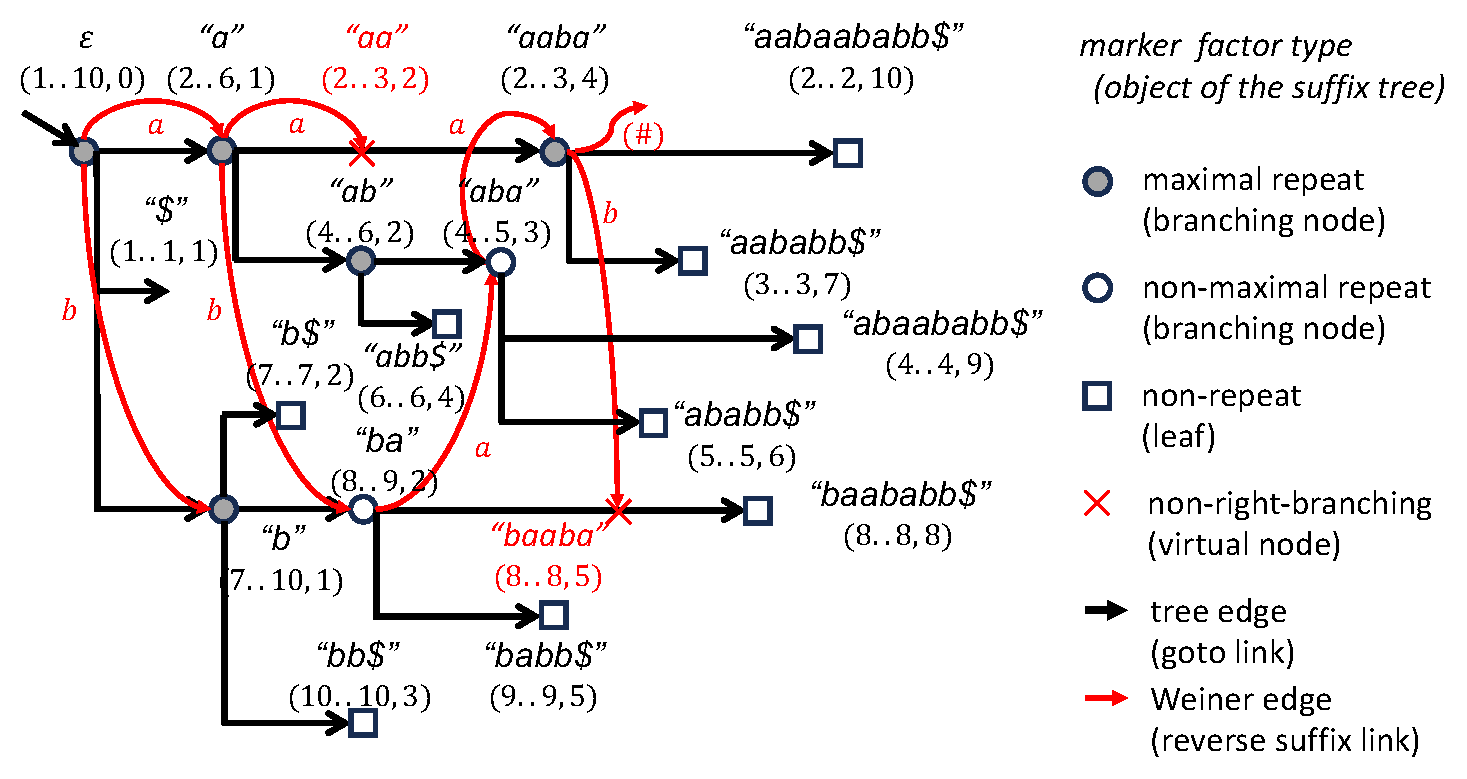
\includegraphics[width=0.7\textwidth]{fig2.pdf}
\vspace{.75\baselineskip}
\caption{An example run of Algorithm $\RecLPT$ for a string $S = \mathtt{aabaababb\$}$, where the left endmarker $S[0]=\#$ and the related suffixes are omitted. 
}\label{fig:run:example}
\end{figure}
%%%%%%


%%%%%%%%%%%%%%%%%%%%%%%%%%%%%%%%%

%% \subsubsection{Computing a set of right-branching characters}
%% %%% 
%% In \cref{algo:genchildren}, we show a procedure $\GenChildren$ for computing the set of all child ranges of an $\ell$-range, based on precomputed arrays $\LCP, \SA, S$.


%% At the top-level, the procedure is invoked with the triple $\pi = (i..j, \ell_*)$ for a factor of $S$ and the pointer to the set $Children = \emptyset$. At every iteration of $\GenChildren[]$, the following pre-condition must be ensured: $\ell_*$ is the lcp-length of all suffixes in the range $i..j$, namely, $RMQ_{LCP}(i+1, j) = \ell_*$ must hold.

%%       %% \If{ $Children = \op{undef}$ }{
%%       %%   We let $Children$ to be the pointer to a newly created set $\emptyset$. 
%%       %% }



%% \begin{toappendix}
%% By definition, we see that
%% $(i,j,\ell) \in \RR$ if and only if
%% \begin{enumerate*}[(i)]
%% \item $k \in i..j \iff u = S[p..p+\ell-1]$ for all $k$, and
%% \item $\ell = minLCP(i,j)$,
%% \end{enumerate*}
%% where $p = SA[k]$ and $minLCP(i,j)$ denotes the minimum LCP-values of an SA-range $i..j$ defined to be $minLCP(i,j) := \max_{i\le k\le j} lcp(S[p..n])$.

%% \begin{remark}[SA-ranges as a representation of right-maximal factors]
%%   We remark that any SA-range $i..j$ without a length component $\ell$ implicitly represents a right-maximal factor of $S$ as follows. By letting $\ell$ to be the min-lcp value of the range, that is, $\ell := minLCP(i,j)$, we obtain the triple $(i..j, \ell)$ representing a $u = S[p..p+\ell-1]$ of $S$, where $p = SA[k]$ with an arbitrary $k \in i..j$. Then, it is not hard to see that $u$ is rigit-maximal in $S$.
%% \end{remark}
%% \end{toappendix}

%% \subsection{Merging dammy leaves to branching nodes (TBD)}

\newpage
%%%%%%%%%%%%%%%%%%
\section{Transforming \LPTrm-tree to CDAWG}
\label{sec:lpt:to:cdawg}
%%%
In this section, we present the second algorithm $\RecCDAWG$ for transforming the \LPTrm-tree $G = (\sig V(G), \sig E(G), root_G)$ for a string $S$ into its CDAWG.
We show the main result of this section.  

\begin{lemma}\label{lem:main:lpt:to:cdawg}
  Let $S$ be any string of length $n$ over $\Sigma$. 
  We can transform the \LPTrm-tree $T$ of $S$ without suffix links into its CDAWG $G$ with suffix links in $O(e_R(S) + e_L(S))$ time and working space, where $e_R(S)$ and $e_L(S)$ are the numbers of right- and left-extensions of maximal repeats in $S$, and an algorithm is allowed to access the read-only copy of the string $S$. 
\end{lemma}

In the above theorem, we remark that the sizes of an input $T$ and the output $G$ are both $O(e_R(S) + e_L(S))$. 

In \cref{algo:rec:cdawg}, we present the psuedo code of $\RecCDAWG$. 
This algorithm performd the breadth-first search of $T$ from the root to leaves using $\sdep(v)$ as the weight of each node $v$. Then, it gradually transforming an input $T = \LPT(S)$ into a partial DAG obtained from $G = \CDAWG(S)$ by merging equivalent nodes into equivalence classes, and adding suffix links between inequivalent nodes. In the following, we will refer to an itermediate DAG $G'$ as a \textit{partial CDAWG} of $S$. When the merging process is done, the resulting partial DAG $G'$ becomes $\CDAWG(S)$.


In the following subsections, we first explain its subroutines. Finally, we present the proof of \cref{lem:main:lpt:to:cdawg} by analyzing the correctness and time complexity of \cref{algo:rec:cdawg}. 

%% \subsection{Outline of the algorithm}
%% \label{sub:outline:recdawg}
%%%
%% In \cref{algo:rec:cdawg}, we present the psuedo code of $\RecCDAWG$. 
%% This algorithm performd the breadth-first search of $T$ from the root to leaves using $\sdep(v)$ as the weight of each node $v$. Then, it gradually transforming an input $T = \LPT(S)$ into a partial DAG obtained from $G = \CDAWG(S)$ by merging equivalent nodes into equivalence classes, and adding suffix links between inequivalent nodes. In the following, we will refer to an itermediate DAG $G'$ as a \textit{partial CDAWG} of $S$. When the merging process is done, the resulting partial DAG $G'$ becomes $\CDAWG(S)$.


%%%%%%%%%%%%%%%%%%
\begin{algorithm}[p]
  \caption{The procedure $\RecCDAWG$ for transforming the \LPTrm-tree $T = (V(T), E(T), root(G))$ of a string $S$ into its CDAWG $G$. 
  }\label{algo:rec:cdawg}
%%%%%%
  %%%
\KwWork{$B\subseteq V(G)\times \nat$: a priority queue of nodes $u$ with $\ldep(u)$ as their weights. $EQ: V(G) \to \pow{V(G)}$: a union-find structure that maps each vertex $u$ to its equivalence class $EQ(u) \in \pow{V(G)}$ with operation $\op{unify}(u, v)$. Tables $\ldep, \sdep: V(G) \to \nat$ that assigns to each node $u$ the string depths of the longest and shortest members in $EQ(u)$ in $T$, respectively. }  
\Begin{ 
\Comment{Initialization}
$B \gets \emptyset$, $\id{suf} \gets \emptyset$, and $wlink \gets \emptyset$\;
Compute the table $\ldep$ by DFS of $T$\; 
\For{each $u \in V(G)$}{
  $\op{nlchar}(u)=|\LChar(\Value(u))|$\Comment*{from the triple of $u$} 
  $EQ(u) = \set{u}$\Comment*{the singleton class}
}
\For{each $f = (u, \alpha, w) \in E(G)$}{
  $B.\op{insert}(f, \ldep(w))$
  \Comment*{Insert $f$ with weight $\ldep(w)\ge 0$}
}
\medskip
\While{ $B \not= \emptyset$}{
  \Comment{Extracting an arc with minimum weight $\ldep(w)$}
  $f = (u, \alpha, w) \gets B.\op{deletemin}()$\;
  \Comment{Finding the locus $v$ of the longest suffix $\beta'$ of the string label $\beta = \Value(u)\cdot\alpha$ such that $\beta' \not\in EQ(\beta)$. }
  $(u', (g_1, \dots, g_k), v) \gets \FindNonEquivLocus(u, \alpha; G, \sdep, \ldep)$\; 
    \label{step:algo2:skip:and:count}
    \Comment{Maintaining links and equivalence class of $v$}
    \uIf (\comblk{Merging two equivalence classes})
         {$\op{nlchar}(v) = 1$}
         %% {$|\wlink(v)| = 0$}
         {
      \Comment{$v$ has no incoming suffix links.}
      $EQ.\op{unify}(w, u)$
       \Comment*{Merging $EQ(w)$ and $EQ(v)$}
      Re-direct all incoming arcs of $v$ into $w$\;
      $\sdep(w) \gets \min\{\sdep(w), \sdep(v)\}$\; 
    }
    \Else (\comblk{Adding suffix and Weiner links between equivalence classes})
    {
      $a = \alpha[\id{offset}]$\Comment*{$\op{shortest}(EQ(w)) = a\cdot \Value(EQ(v))$}
      $\id{suf}(w) \gets v$\Comment*{an incoming suffix link to $v$}
      $\wlink(v, a) = v$\Comment*{an explicit W-link from $v$}
      %% Add , namely, , and  with character $a$, namely, , where  is the first character of the shortest emember of $EQ(w)$, that is, . \; 
    }
} %% While
\Return the CDAWG $G = (V(T), E(T), root(G), \id{suf}, \wlink)$ of $S$\; 
}%Begin
%%%%%%
\end{algorithm}
%%%%%%%%%%%%%%%%%%




%% We show a few technical lemmas below. Let $G'$ be a partial CDAWG obtained from $\LPT(S)$ by merging a subset of equivalent nodes with respect to the equivalence relation $\eqepos$ on $\Sub(S)$. 

%% \begin{lemmarep}\label{lem:trans:cdawg:one}
%% Let $\alpha, \beta \in \Sub(S)$ be any factors of $S$ such that $\alpha$ is a suffix of $\beta$, i.e. $\beta \succeq^\idrm{suf} \alpha$. In $\CDAWG(S)$, if the locus of $\beta$ is an explicit node of $G'$, then so is the locus of $\alpha$. 
%% \end{lemmarep}

%% \begin{proof}
%%   Recall that a locus $\loc u$ is an explicit node in
%%   $\CDAWG(S)$
%%   if and only if
%%   $|\Epos(u)| \ge 2$.
%%   Since $\beta \succeq^\idrm{suf} \alpha$, we have $|\Epos(\alpha)| \ge |\Epos(\beta)| \ge 2$. 
%% \end{proof}

\subsection{Preprocessing $\op{ldep}(u)$ and $\sdep(u)$ in $O(e_R)$ total time}
\label{sec:compute:cdawg:preprocess}

During the computation, we incrementally compute the the pair $(\op{ldep}(u), \sdep(u))$ of quantities on the \LPTrm-tree, defined as follows. 
 %% and $\op{shortdep}(u)$ of the longest and shortest paths from the root to $u$ are already computed, where
\begin{itemize}
\item $\op{ldep}(u)$ is the \textit{largest string depth}, defined to be the length of the longest paths from the root to $u$,
that is, $\ldep(u) = \max \sete{ |\str(\pi)| : \pi \in Path(root, u) }$

\item $\sdep(u)$ is \textit{the smallest string depth}, defined to be the length of the longest paths from the root to $u$, that is, $\sdep(u) = \min \sete{ |\str(\pi)| : \pi \in Path(root, u) }$. 
\end{itemize}

Clearly, $\ldep(u) = |\Value(u)|$.
The fields for the above information require $O(\mu(S))$ space. 
Then, the computation of the the pair $(\op{ldep}(u), \sdep(u))$ is done by the following recurrences. 
\begin{lemma}\label{lem:ldep:sdep:rec}
Let $G$ be the CDAWG  of a string $S$ and $u$ be any of its explicit node. 
\begin{enumerate}
\item If $u$ is the root of $G$, $\ldep(u) = \sdep(u) = 0$. 
  
\item Otherwise, $u$ is an explicit node with one or more incoming arcs $f_1, \dots, f_k$ such that $\dst(f_i) = u$ for all $\btw i1k$ and $k\ge 1$.
Then, we have 
  \begin{itemize}
  \item $\ldep(u) = \max{}\idx i1k \{\: \ldep(\src(f_i)) + |\lab(f_i)|  \:\}$
  \item $\sdep(u) = \min{}\idx i1k \{\: \sdep(\src(f_i)) + |\lab(f_i)|  \:\}$
  \end{itemize}
  where $f_i = (\src(f_i), \lab(f_i), \dst(f_i)) = (v_i, \alpha_i, u) \in V(G)\by\Sigma^+\by V(G)$. 
\end{enumerate}
\end{lemma}

From \cref{lem:ldep:sdep:rec}, the total computation can be done in $O(e_R(S)+e_L(S))$ time and $O(\mu(S))$ working space on the CDAWG of $S$. 
We remark that \cref{lem:ldep:sdep:rec} holds even for a partial CDAWG $G$ whenever the current node $u$ has been merged to all of its equivalent nodes and all ancestors have been processed so far.

  We assume that the Boolean flag $\op{nlchar}(v) \iffdef |\LChar(\Value(v))|\ge 2$ is attached to each explicit node $v$ in $T$. This can be  computed from the triple for $\Value(v)$ by $\isLeftBranching(i..j, \ell)$ of \cref{lem:leftmaximal:character} in the procedure $\RecLPT$. 



%%%%%%%%%
\subsection{Computation of the locus of the longest non-equivalent prefix of the representative string}
\label{sec:compute:cdawg:equiv:classes}
%%
In the CDAWG of $S$, there exists a suffix link between the representatives $\beta$ and $\beta'$ of two equivalence classes such that $|\beta| > |\beta'|$ if and only if $\beta'$ is the longest suffix of $\beta$ that does not belong to the equivalence class of $\beta$.
Therefore, it is sufficient to find the locus $v$ of such $\beta'$ from the locus $w$ of $\beta$. Then, we have the next lemma. 


\begin{lemma}\label{lem:find:ne:locus}
  %%\textit{Claim}~2.
  During the computation of a partial CDAWG of $S$ from $\LPT(S)$, 
  the computation of the target $v$ and the arcs $g_1, \dots, g_k$ can be done in $O(e_R(S)+e_L(S))$ total time over all arcs $f$ using the procedure  $\FindNonEquivLocus$ in \cref{algo:find:ne:locus}. 
\end{lemma}


\begin{toappendix}
In \cref{algo:find:ne:locus}, we show the procedure $\FindNonEquivLocus(u, \alpha; G, \sdep, \ldep)$ that computes the locus $v$ of the longest suffix $\beta'$ of the string label $\beta = \Value(u)\cdot\alpha$ such that $\beta' \not\in EQ(\beta)$, and the associated path $(g_1, \dots, g_k)$ from a node $u'$ to $v$.
See \cref{fig:three:suffix:link} for the explanation of the procedure.

%%%%%%
\begin{figure}[t]
\centering
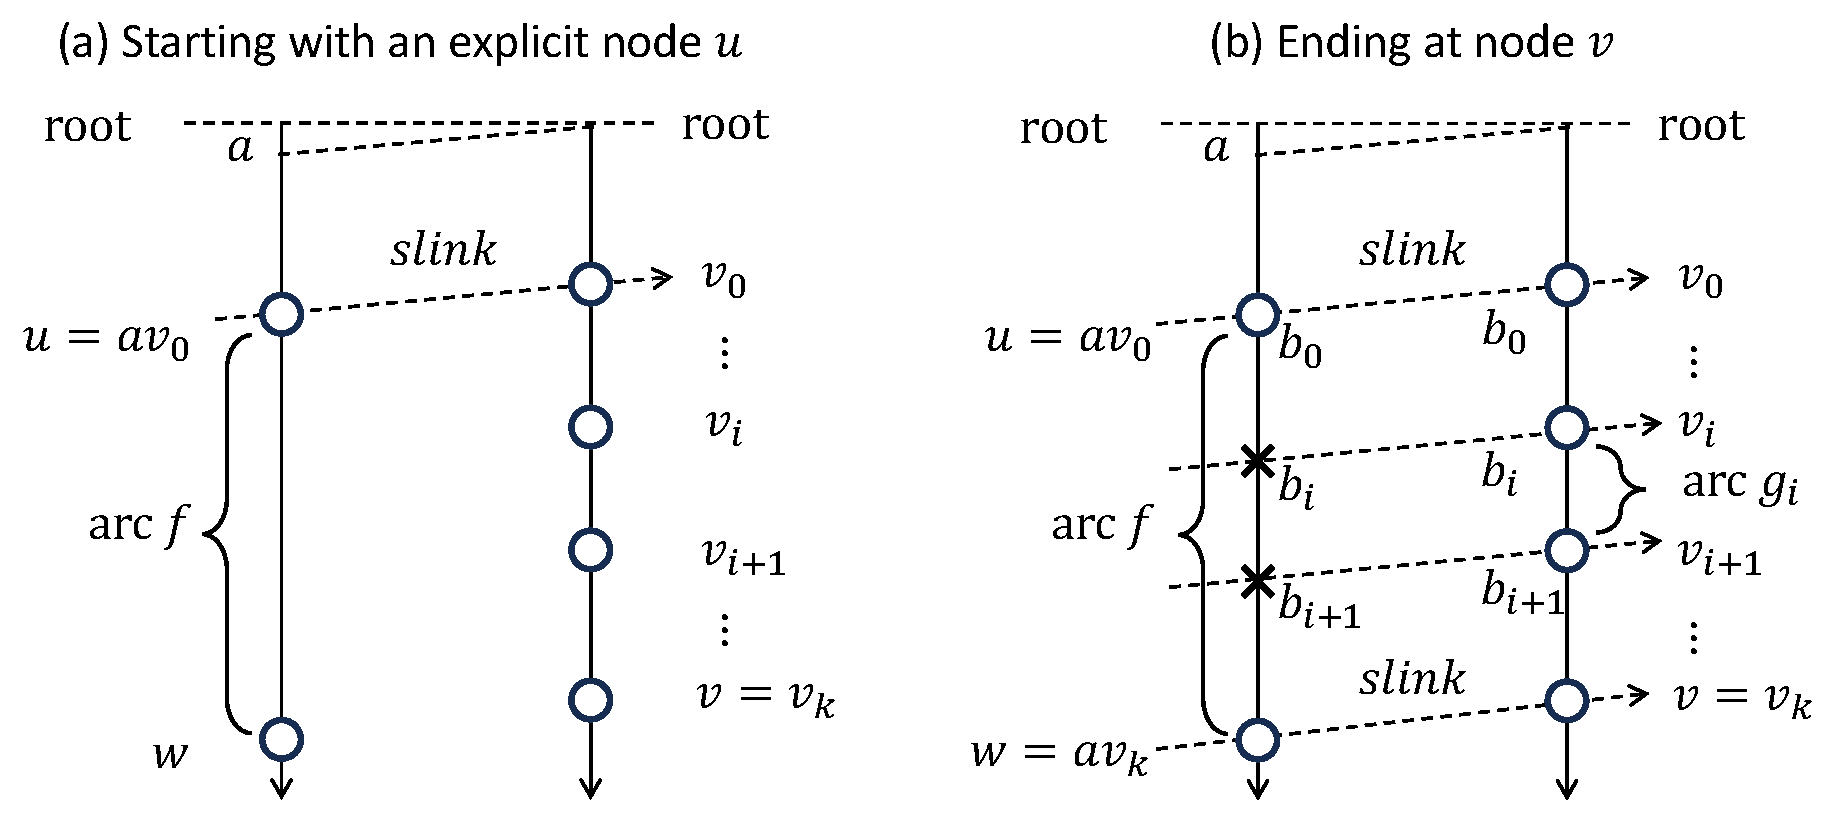
\includegraphics[height=0.4\textwidth]{fig3.pdf}
\vspace{.5\baselineskip}
\caption{Explanation of the procedure $\FindNonEquivLocus(u, \alpha; G, \sdep, \ldep)$ in \cref{algo:find:ne:locus}. Given the string label $\alpha = \lab(f)$ of an arc $f = (u, \alpha, w)$, it finds the locus $v$ of the shrinked string $\alpha' = \alpha[1+\id{offset}..|\alpha|]$. This can be done in total time $O(e_L(S) + e_R(S))$ using the so-called skip-and-count technique.}
\label{fig:three:suffix:link}
\end{figure}
%%%%%%

  
%%%%%%%%%%%%%%%%%%
\begin{algorithm}[t]
  \caption{
The procedure $\FindNonEquivLocus(u, \alpha; G, \sdep, \ldep)$ that computes the locus $v$ of the longest suffix $\beta'$ of the string label $\beta = \Value(u)\cdot\alpha$ such that $\beta' \not\in EQ(\beta)$, and the associated path $(g_1, \dots, g_k)$ from a node $u'$ to $v$. 
  }\label{algo:find:ne:locus}
  %%%%%%
  \Comment{Computing the initial node $u'$ and a suffix $\alpha'$ of $\alpha$}
  \uIf{$u = root(G)$}{
    $(u', \id{offset})\gets (root(G), 1)$\; 
  }
  \Else{
    $(u', \id{offset})\gets (\id{suf}(u), \ldep(u) - \sdep(u) + 1)$\; 
  }
  $\alpha' \gets \alpha[\id{offset}..|\alpha|]$\; 
  %%%
  %%At stage $i=0$, we initialize the target length by
  \Comment{Finding a path $(g_1, \dots, g_k)$ with skip-and-count}
  $\ell_* \gets |\alpha|$; $\ell \gets 0$; $v_0 \gets v$; $i \gets 0$\;     
  \While{$\ell < \ell_*$}{
    $b_i \gets \alpha[\ell + 1] \in \Sigma$\Comment*{a branching character}
    $g_i = (v_{i-1}, \beta_i, v_i) \gets \Out(v_{i-1}, b_i)$\; 
    $\wlink(v_i, a) \gets f$\Comment*{Adding a new implicit W-link}
    $\ell \gets \ell + |\beta_i|$; $i \gets i+1$\; 
  }
  \Return $(u', (g_1, \dots, g_k), v)$, where $k = i-1$\; 
\end{algorithm}
%%%%%%%%%%%%%%%%%%
\end{toappendix}

\subsection{Analysis}
%% \subsection{The proof of \cref{lem:main:lpt:to:cdawg}}

Consider the psuedo code of the procedure $\RecCDAWG$ in \cref{algo:rec:cdawg}.

\begin{lemmarep}[correctness]\label{lem:cdawg:correctness}
  Let $T$ be the $\LPT(S)$ of a string $S$ of length $n$. 
  We assume that $\op{nlchar}(v) = |\LChar(\Value(v))|$ is attached to each explicit node $v$ in $T$. Then, \cref{algo:rec:cdawg} correctly computes $\CDAWG(S)$ from $T$ and $S$. 
\end{lemmarep}

\begin{proof}
Suppose that initialization of Lines 2--6 are done. 
We introduce some notion as follows.
Consider any iteration of the while-loop for Lines 7--17 of \cref{algo:rec:cdawg}.
Let $w$ be any explicit node in $V(T)$.
\begin{itemize}
\item We define the total order $\preceq$ on $V(G)$ as $u \preceq v \iffdef \ldep(u) \le \ldep(v)$, and its strict version $\prec$. 
\item For any explicit node $w$, we denote $V\rk{\preceq w}(T) := \sete{ v \in V(T) \mid \ldep(v) \le \ldep(w) }$ be the subset of all nodes $v$ with $\ldep(v) \le \ldep(w)$.
  
\item We let $\eqepos[\preceq w]$ be the subrelation of $\eqepos$ restricted to $V\rk{\preceq w}(T)$, namely, $(\eqepos[\preceq w]) = \sete{ (u,v) \in (\eqepos) \mid u, v \in V\rk{\preceq w}(T)}$, and $[u]^{\preceq w}_{\equiv}$ be the associated equivalence class with representative $u$.

\item Similarly, we let $\eqepos[\prec w]$ and $[u]^{\prec w}_{\equiv}$ as the subrelation and equivalence class with $\prec w$ instead of $\preceq$, respectively. 
\end{itemize}

At the timing where a new arc $f = (u, \alpha, w)$ with weight $\ldep(w)$ is extracted from $B$, we remark that $\eqepos[\prec w]$ and $\eqepos[\preceq w]$ correspond the node subsets $V\rk{\preceq w}\setminus\set{w}$ and $V\rk{\preceq w}(T)$, respectively. We will show the following claim.

\textit{Claim~1}: At any iteration of the while-loop for Lines 7--17 of \cref{algo:rec:cdawg}, suppose that a new arc $f = (u, \alpha, w)$ with weight $\ldep(w)$ is extracted from the priority queue $B$. Then, in the end of the iteration at Line 17, the following conditions hold:  
\begin{enumerate}
  \item For all explicit nodes $w'$ in $V\rk{\preceq w}(T)$ with $\ldep(w') \le \ldep(w)$, $EQ(w') = [w']^{\preceq w}_{\equiv}$ holds and $w'$ has an outgoing suffix link.
  \item For all explicit nodes $w'$ with $\ldep(w') < \ldep(w)$, $w'$ has a soft-Weiner link $\wlink(w', a) = g$ for some character $a$ and an arc $g$ if the string $a\cdot\Value(w')$ is a factor of $S$. 
\end{enumerate}


Consider condition (1). Let $f = (u, \alpha, w)$ be the new arc with weight $\ldep(w)$ is extracted from $B$ in the beginning of the while-loop.
We will show the claim that at the end of the while-loop, the equivalence relation $\eqepos[\preceq w]$ and the associated equivalence classes are correctly maitained on the updated domain $V\rk{\preceq w}(T) = V\rk{\prec w}(T) \cup \set{w}$. 

Suppose first that there exists another node $v$ in $V\rk{\prec w}(T)$ such that $[v]^{\prec w}_{\equiv} \not= [w]^{\prec w}_{\equiv}$ and $\Value(w) \succeqsuf \Value(v)$ (*) in the beginning of the while-loop. Note that we use $\prec w$ instead of $\preceq w$. Then, we see that $\ldep(v) < \ldep(w)$ othewise they must be identical. 
Among such $v$'s, we choose the deepest $v$ with largest $\ldep(v)$ in $V\rk{\preceq w}(T)$ with property (*).
From \cref{lem:find:ne:locus}, we can find the locus $v$ by calling $\FindNonEquivLocus$ with arguments $u$ and $\alpha$ at Line~9 of \cref{algo:rec:cdawg}. 
%%we can find such a node $v$ with the string label $\beta' = \Value(v)$ by using the procedure $\FindNonEquivLocus$. 


Let $\beta$ and $\beta'$ be the string labels of $w$ and $v$, respectively. Then, we can show that $\beta'$ is the longest suffix of $\beta$ such that $\Epos(\beta) \not= \Epos(\beta')$.
There are two cases (a) and (b) below on the current equivalence relation $\eqepos[\preceq w]$ instead of $\eqepos[\prec w]$. 
\begin{enumerate}[(a)]
\item If $\beta \eqepos[\preceq w] \beta'$ holds, since $\beta \succsuf \beta'$, we can show that this condition is equivalent to $|\LChar(\beta')| = \op{nlchar}(v) \ge 2$, which can be correctly detected at Line 10. 
  the equivalence classes $[w]^{\prec w}_{\equiv}$ and $[v]^{\prec w}_{\equiv}$ of $\beta$ and $\beta'$, respectively, must be merged into the new class $[w]^{\preceq w}_{\equiv}$. This is done by the code for Lines 11--13. 
  
\item Otherwise, $\beta \not\eqepos[\preceq w] \beta'$ holds. By the same argument as (a), this condition is equivalent to $|\LChar(\beta')| = \op{nlchar}(v) = 1$, which can be correctly detected at Lines 10 and 14.
  the equivalence classes $[w]^{\prec w}_{\equiv} = [w]^{\preceq w}_{\equiv}$ and $[v]^{\prec w}_{\equiv} = [v]^{\preceq w}_{\equiv}$  of $\beta$ and $\beta'$, respectively, must remain separated, and the suffix link from $w$ to $v$ must be added, where $\id{offset} = |\beta| - |\beta'|$ and $a = \alpha[\id{offset}]$. 
  This is correct because $[v]^{\prec w}_{\equiv}$ is the predecessor of $[w]^{\prec w}_{\equiv}$ w.r.t.~the suffix relation $\succsuf$ on their values.
\end{enumerate}

Combining the above arguments, at the end of the while-loop, we have correctly maintained the equivalence relation $\eqepos[\preceq w]$ and the associated equivalence clases on the updated domain $V\rk{\preceq w}(T) = V\rk{\prec w}(T) \cup \set{w}$.
\end{proof}

Next, we consider the time complexity. 

\begin{lemmarep}[time and space complexity]\label{lem:cdawg:complexity}
  Given $\LPT(S)$ of a string of length $n$, 
  \cref{algo:rec:cdawg} runs in $O(e_R(S) + e_L(S) + \mu(S)\log \mu(S))$ time and $O(e_L + e_R)$ space. 
\end{lemmarep}

\begin{proof}
Let us denote by $\mu = \mu(S), e_R = e_R(S)$, and $e_L = e_L(S)$, where $\mu \le \min\{e_R, e_L\}$.
In the initialization for the tables $EQ$, $\ldep$, $B$ for Lines 2--8 can be done in $O(e_R)$ total time. The precomputation of the table $\op{nlchar}$ at Lines 7--8 can be done in $O(e_L)$ total time by computing $\LChar(\tau)$ with the associated triple $\tau$ stored in $u$. 
In each iteration of the while-loop, $\op{deletemin}$ on the priority queue requires $O(\mu \log \mu)$ total time over all of $\mu$ nodes using $O(\mu)$ space on the standard heap.
From \cref{lem:find:ne:locus}, the call of $\FindNonEquivLocus$ at Line~9 requires $O(e_R + e_L)$ total time. Redirection of all incoming arcs of $v$ into $w$ at Line 13 can be done in $O(e_R)$ since $v$ has exactly once suffix link since it is equivalent to $w$, and thus it is not left-branching.
Additions of the suffix and Weiner links for Lines 18--19 can be executed at most the number of suffix links, and are bouned in $O(e_L)$ time.
\end{proof}

\begin{trivlist}\item[]
  \textbf{Proof of \cref{lem:main:lpt:to:cdawg}:}
  Combining \cref{lem:cdawg:correctness} and \cref{lem:cdawg:complexity}, \cref{lem:main:lpt:to:cdawg} immediately follows.
\qed   
\end{trivlist}

\begin{trivlist}\item[]
  \textbf{Proof for \cref{thm:main:index:cdawg}}.
  Combining 
  \cref{lem:main:from:lpt:to:cdawg:correct:time}
  and
  \cref{lem:main:lpt:to:cdawg}, we can show \cref{thm:main:index:cdawg}. 
\qed
\end{trivlist}



%% In \cref{algo:rec:cdawg}, we present the psuedo code of $\RecCDAWG$, which gradually transforms $T = \LPT(S)$ to $G = \CDAWG(S)$ by performing breadth-first search of $T$ from the root to leaves. 
%% During BFS, it adds suffix links between inequivalent nodes and merges equivalent nodes into equivalence classes. 
%% %% Our algorithm incrementaly computes suffix links and equivalence classes by
%% %% performing depth-first search from the root to leaves in the \LPTrm-tree. 
%% We will refer to an itermediate DAG $G'$ obtained form the \LPTrm-tree after merging a subset of equivalent nodes as a \textit{partial CDAWG} of $S$. When the merging process is done, the resulting partial DAG $G'$ becomes $\CDAWG(S)$.

%% Below, we show the details of \cref{step:algo2:skip:and:count} in the above algorithm. The traversal can be done in $O(k)$ time using constant time per arc, by the skip-and-count technique as follows (see \cref{fig:three:suffix:link}).e

%% %%%%
%% \begin{enumerate}
%%   \item  
%%     Select the triple $(v, \id{offset}, \alpha')$ of the initial node $v \in V(G)$, a positive integer $\id{offset} \in \nat$, and a prefix $\alpha'$ of $\alpha$ as follows. Let $u = \src(f)$ be the source of arc $f$: 
%%     \begin{enumerate}[(i)]
%%     \item If $u$ is the root, we let $v := root(G)$, and $\id{offset} := 1$. 
%%     \item Otherwise, $u$ is an explicit node other than the root, with the suffix link $\id{suf}(u)$. Moreover, the pair $(\ldep(u), \sdep(u))$ has been computed. Then, we let $v$ to be the target of the suffix link, $v := \id{suf}(u)$, and let $\id{offset} := \ldep(u) - \sdep(u) + 1$. 
%%     \end{enumerate}
%%     Finally, we shrink the label of $\alpha$ by $\id{offset}$ character length, that is, $\alpha' := \alpha[1+\id{offset}..|\alpha|]$.
%%     The intended meaning of $\alpha'$ is the longest suffix of the representative $\Value(u)$ that do not belong to the equivalence class of $u$.
%% \end{enumerate}
%% %%%%



%% %%%%%%%%%
%% \subsection{$O(e_R)$-time Computation of the Equivalence Classes}
%% \label{sec:compute:cdawg:equiv:classes}
%% %%% 
%% %%Then, the algorithm computes the suffix link of explicit nodes, and all inplicit W-links into all type-2 nodes (loti) by breadth-first traversal of the \LPTrm-tree. We make the following inductive assumption. 
%% %We first performs the base case, and then induction cases. Finally, return the revised graph $G = (\sig V, \sig E, root, \wlink, \id{suf})$.

%% In \cref{line:recdag:one}, by induction hypothesis, $w$ is an explicit node whose target $w$ has the smallest string depth $\ell = \ldep(w)$ among the targets of all unprocessed arcs in $B$. This implies the next claim. \; 
%% \begin{enumerate}[(1)]
%%   \item 
%%     \begin{itemize}
%%     \item \textit{Claim}~1. All node in $V(T)$ with string length strictly less than $\ell$ are already processed as follows. If $u$ is not the root, it has a suffix link $\id{suf}(u)$ to another explicit node. Furthermore, it is already merged into the equivalence class $EQ(u')$ of a smaller string depth $\ldep(u')$ equivalent to $u$, i.e., $u \eqepos u'$. 
%%     \end{itemize}
%% \end{enumerate}



%% %%%%%%
%% \mysubsubsection{The base case. We perform the following initialization.}
%% %%%
 
%% \begin{itemize}
%% \item We let $B \gets E(G)$, $suf \gets \emptyset$, and $wlink \gets \emptyset$.
  
%% \item For all nodes $u$ in $V(G)$, we let $EQ(u)$ be the singleton class, i.e., $EQ(u) = \set{u}$. 
%% %% \item Insert all outgoing arcs $f \in \Out(root(G))$ of the root into $B$ with weight $w = \ldep(\dst(f))$.
%% \end{itemize}

%% \mysubsubsection{The induction case.}
%% %%%
%% As induction hypothesis, we assume that whenever an edge $f \in \sig E(G)$ is extracted from the queue $B$, its source $u = \src(f)$ satisfies that: either (i) the source $u$ is the root of $G$, or (ii) $u$ has the suffix link $v = \id{suf}(u)$ with some $v \in \sig V(G)$.
%% Then, we process all arcs in $\sig E(G)$ by executing the following steps while $B \not= \emptyset$: 
%% \begin{enumerate}[(1)]
%%   \item 
%%     Firstly, we extract from the priority queue $B$ a new edge $f = (u, \alpha, w)$ with the minimum weight $\ldep(w)$.
%%     By induction hypothesis, $w$ is an explicit node whose target $w$ has the smallest string depth $\ell = \ldep(w)$ among the targets of all unprocessed arcs in $B$. This implies the next claim. 
%%     \begin{itemize}
%%     \item \textit{Claim}~1. All node in $V(T)$ with string length strictly less than $\ell$ are already processed as follows. If $u$ is not the root, it has a suffix link $\id{suf}(u)$ to another explicit node. Furthermore, it is already merged into the equivalence class $EQ(u')$ of a smaller string depth $\ldep(u')$ equivalent to $u$, i.e., $u \eqepos u'$. 
%%     \end{itemize}
%%     Let $\beta = \Value(u)\cdot \alpha$ the string label of the longest path from the root to $w$ through the arc $f$. Then, if $w$ is an explicit node, then so is $v$ since 
%%     Note that we do not explicitly compute the string label $\beta$.

%%   \item 
%%     Next, we let $\beta'$ be the longest suffix of $\beta$ such that $\beta'$ is not included in the equivalence class $EQ(\beta)$ of $\beta$. Then, we can quickly find the locus $v$ of $\beta'$ by traversing the list of consecutive arcs arcs $g_1, \dots, g_k$ spelling the string label $\lab(g_1)$ $\cdots$ $\lab(g_k) = \beta'$ along the unique path from the root to the locus $v$ of the prefix $\beta'$. 
%%     \label{step:algo2:skip:and:count}
%%     \begin{itemize}
%%     \item \textit{Claim}~2. The computation of the target $v$ and the arcs $g_1, \dots, g_k$ can be done in $O(e_R(S)+e_L(S))$ total time over all arcs $f$ as shown later.
%%     \end{itemize}

%%   \item Finally, we maintain the suffix link and equivalence class of $v$ as follows.
%% By induction hypothesis, we know that the node $v$ is already processed since $\ldep(v) < \ldep(w)$. Then, there are two cases below on the number of suffix links incoming to the target $v$ (this can be checked by $|\wlink(v)|$). 
%%    \begin{enumerate}[(a)]
%%    \item In the case that $|\wlink(v)| = 0$, namely, $v$ has no incoming suffix links. Then, we merge $v$ into the target $w$ of arc $f$ by re-directing all incoming arcs of $v$ into $w$. Moreover, we update the length $\sdep(w)$ of the shortest path to $w$ with $\min\{\sdep(w), \sdep(v)\}$. 

%%    \item Otherwise, add an incoming suffix link to $v$, namely, $suf(w) = v$, and an explicit W-link from $v$ with character $a$, namely, $\wlink(v, a) = t$, where $a = \alpha[\id{offset}]$ is the first character of the shortest emember of $EQ(w)$, that is, $\op{shortest}(EQ(w)) = a\cdot \Value(EQ(v))$. 

%%    %% \item Finally, in both cases, we add all arcs $f'$ outgoing from $v$ into $B$ with the weight $\ldep(\dst(f'))$.
%%    \end{enumerate}
%%   \end{enumerate}
%% %%%%%%


%% %Computation of suffix and Weiner links 
%% %%%%%%

%% \begin{remark} In (2) (iii) (b), This search for a $b_i$-arc always succeeds. 
%% \end{remark}

%% \begin{proof}
%%   We can show the next claim by construction of $\LPT(S)$. 
  
%%   \textit{Claim~1.} Consider $a u \in L(G)$ for some $a \in \Sigma$ and $u \in \Sigma^*$. If $u \not\in L(G)$, then there exists some factorization $u = pq$ with some $p, q \in \Sigma^*$ such that prefix $p$ is equivalent to $ap$, i.e., $\Epos(ap) = \Epos(p)$. (End of Claim~1)

%% In Claim~1, the prefix $p$ is not left-brancing since we have a left-extension $ap$ of $p$ with the same end-positions. Therefore, the traversal from the initial node $v$ to $u = pq$ terminates at the locus of $p$ when the mergi of $\loc p$ into $\loc {ap}$ happened. 
%% \end{proof}





%% Consider the extended LPT tree of $S$, $\LPT(S) = (\sig V(S), \sig E(S), \eps)$. We introduce the set $\sig W(S)$ of Weiner-links as follows. 
%% For any node $\underline u \in \sig V(S)$ with string labels $u$, and any character $a \in \Sigma$, if $v = au$ is a factor of $S$, $au \in \Sub(S)$, we put the (either soft or hard) Weiner link $g = (\underline u, \underline v)$ from $\underline u$ to the locus $\underline v$ of $v$ with character label $\lab(g) = a$ in $\LPT(S)$. Then, we say that $u$ is the parent of $v$, and $v$ is a child of $u$ w.r.t.~$\sig W(S)$. 
%% Moreover, the link $g$ is \textit{hard} if $\underline v$ is a real (right branching) node, and \textit{soft} otherwise (that is, $\underline v$ is a locus on an arc).
%% %% 
%% We can easily show that the total number of hard and soft Weiner links are upperbounded by the number $e_L$ of left-extensions of maximal repeats of $S$. 

%% Without loss of generality, we identify the triples and the nodes of $\LPT(S)$. Based on the above definition of $\sig W(S)$ and its parent-child relation, we show the next lemma, which is the dual of \cref{lem:prune:leftbranch}. 

%% \begin{lemma}\label{lem:prune:rightbranch}
%% Suppose that a triple $\pi$ is the parent of a triple $\tau$ with respect to the Weiner links in $\sig W(S)$. If the substring $au$ defined by $\tau$ is right-branching, the substring $u$ defined by $\pi$ is also right-branching. 
%% \end{lemma}

%% \begin{proof}
%%   By symmetry, the lemma follows from the proof of \cref{lem:prune:leftbranch}. 
%%   %% If $v = au$ for some $a \in \Sigma$, we can easily show that
%%   %% $\RChar(au) \subseteq \RChar(u)$, and thus that $|\RChar(au)| \le |\RChar(u)|$. On the other hand $au$ is right-brancing in $S$ if and only if $2\le |\RChar(au)|$. It immediately follows that $2 \le |\RChar(u)|$ meaning that $u$ is right-brancing in $S$. This shows the lemma. 
%% \end{proof}

%% Recall that $\sig V$ is the set of nodes for all maximal repeats in $\MR(S)$ and $\eps \in \sig V$. 
%% We let $\sig W$ to be the set of all Weiner links $g = (\underline u, \underline{au})$ that connect elements of $\sig V$ with a character $a \in \Sigma$, that is, $\set{u, au} \subseteq \MR(S)$.

%% Now, we define the \textit{Weiner-link counterpart} of $\LPT(S)$, denoted by $\LPT[-](S) = (\sig V_-, \sig W_-, \eps)$ as follows.
%% \begin{itemize}
%% \item $\sig F_- = \sete{ g = (\underline u, \underline au) \mid u\in\MR(S), u\not\in \MR(S) }$ is the set of all Weiner links $g = (\underline u, \underline au)$ that connect maximal nodes of $\sig V$ to non-maximal nodes. 
%%   %%, that is, $u\in\MR(S)$ and $u\not\in \MR(S)$.
%% \item Let $\sig V_- = \sig V \cup \Delta_-$, 
%%   where $\Delta_- = \sete{\underline{au} \not\in\sig V \mid g = (\underline u, \underline{au}) \in \sig F_-}$ be the set of non-maximal nodes reachable from $\sig V$ by arcs of $\sig F_-$.
  
%% \item $\sig W_+$ be the union of $\sig W$ and $\sig F_-$. 
%% \end{itemize}

%% Then, the extend LPT tree w.r.t.~Weiner links in $\sig W$ is the rooted tree $\LPT[-](S) = (\sig V_-, \sig W_-, \eps)$. 


%% \subsection{Putting it all together}
%% %%%

%% Suppose that an index $\sig I = (\SA, \ISA, \LCP, S)$ is preprocessed from $SA$ and $S$ in \cref{algo:main}. 
%% Consider the recursive procedure $\RecLPT$ in \cref{algo:rec}, which is equipped with subprocedure $\GenChildren$ in \cref{algo:genchildren} and the procedure $\isLeftBranching(i..j, \ell)$ in \cref{lem:leftmaximal:character}. 

%% \subsection{$O(e_{\max})$-worst-case time solution over a constant alphabet}

%% From
%% \cref{lem:maxrep:howto:child},
%% \cref{lem:genchildren},
%% \cref{lem:leftmaximal:character},
%% and the construction of $\LPT(S)$, 
%% the recursive procedure $\RecLPT$ in \cref{algo:rec} correctly construct all nodes and edges of $\LPT(S) = (\sig V(S), \sig E(S), \eps)$ by generating all maximal repeats by starting with the root $\eps$, and by following all arcs $(u, v)$ in $\E(S)$ defined with the right-closure $v = \rext{(ub)}$ of a right-extension $ub$ with a branching character $b$ using a depth-first traversal of $\LPT(S)$.
%% From \cref{lem:prune:leftbranch}, we see that if it eventually reaches a non-maximal node in $\Delta(S)$, it correctly stops the search and backtracks. Each arc is added to the arc set whenever it is traversed. Since each node $\underline v$ in $\E(S)\cup \F(S)$ can be reached through exactly one incoming arc, the procedure correctly find all arcs.


%%%% 
\section{Conclusion}
\label{sec:concl}
In this paper, we consider the problem of transforming the suffix array $\SA$ of a string $S$ of length $n$ to its CDAWG $G$. Then, we  presented a simple and efficient algorithm for solving this problem in $O(e_R + e_L + \mu\log n)$ time  based on $\SA$, $\ISA$, and $\LCP$ arrays of $S$ with the RMQ structures of $O(n)$ size.
It is a future work to implement the proposed algorithm on the existing implementation of succinct and self-index structures for a string, and to evaluate its performance on highly-repetitive strings in the realworld. 


%%%% end of body %%%%%%%%%%%%%%%%%%

% ---- Bibliography ----
\newpage
\bibliographystyle{plain}
\bibliography{ref}
%% \bibliography{bib/ref,ref}
\end{document}

